\hypertarget{einleitung}{%
\section{Einleitung}\label{einleitung}}

\hypertarget{motivation}{%
\subsection{Motivation}\label{motivation}}

\begin{itemize}
\tightlist
\item
  Beginn: Er zieht die Aufmerksamkeit des Lesers durch die Schilderung
  des Ereignisses auf sich, das zu dem Problem geführt hat.
\item
  Hintergrundinformationen (Herstellung des Kontexts): Gehe tiefer auf
  das Ereignis ein, indem du mehr Informationen über es vermittelst und
  dabei auch den Rahmen deiner Forschung skizzierst.
\item
  Brücke zur Problemstellung: Erläutere, inwiefern es sich hierbei um
  ein Problem handelt, und schlage somit die Brücke zur Problemstellung,
  die deiner Untersuchung zu Grunde liegt.
\end{itemize}

\hypertarget{zielsetzung}{%
\subsection{Zielsetzung}\label{zielsetzung}}

Das Ziel dieser Arbeit ist es, einen autonomen Schachtisch zu
entwickeln, welcher in der Lage ist Schachfiguren autonom zu bewegen und
auf Benutzerinteraktion zu reagieren. Der Schwerpunkt liegt dabei
insbesondere auf der Programmierung des eingebetteten Systems und dem
Zusammenspiel von diesem mit einem aus dem Internet erreichbaren
Servers, welcher als Vermittlungsstelle zwischen verschiedenen
Schachtischen und anderen Endgeräten dient. Dieses besteht zum einem aus
der Positionserkennung und Steuerung der Hardwarekomponenten
(Schachfiguren) und zum anderen aus der Kommunikation zwischen dem Tisch
selbst und einem in einer Cloud befindlichem Server. Mittels der
Programmierung werden diverse Technologien von verschiedenen
Einzelsystemen zu einem Gesamtprodukt zusammengesetzt.

\hypertarget{methodik}{%
\subsection{Methodik}\label{methodik}}

Im ersten Abschnitt werden die zum Zeitpunkt existierenden Ansätze und
deren Umsetzung beleuchtet. Anschliessend werden die zuvor verwendeten
Technologien betrachtet, welche bei bei den beiden darauffolgenden
Prototypen verwendet wurden.

Das sechste Kapitel widmet sich der realisierung des erste Protoypen des
autonomen Schachtischs. Dabei werden alle Im anschliessenden Kapitel,
wird auf der Basis des ersten Prototyps und seiner auftretenden
Probleme, der finale Prototyp entwickelt. Hier werden die Probleme durch
ein re-design und vereinfachung der Elektronik gelößt und so ein
zufriedenstellendes Produkt entwickelt.

Im darauffolgenden Abschnitt wird die Cloud-Infrastruktur thematisiert,
welche für eine Kommunikation zwischen den Prototypen entscheidend ist.

\begin{itemize}
\tightlist
\item
  controller software
\item
  fazit
\end{itemize}

\hypertarget{analyse-bestehender-systeme-und-machbarkeitsanalyse}{%
\section{Analyse bestehender Systeme und
Machbarkeitsanalyse}\label{analyse-bestehender-systeme-und-machbarkeitsanalyse}}

\hypertarget{existierende-systeme-im-vergleich}{%
\subsection{Existierende Systeme im
Vergleich}\label{existierende-systeme-im-vergleich}}

\begin{itemize}
\tightlist
\item
  Nischenprodukt, jedoch einige Projekte im OpenSource bereich verfügbar
\item
  Ein kommerzieller Hersteller
\end{itemize}

\hypertarget{kommerzielle-produkte}{%
\subsubsection{Kommerzielle Produkte}\label{kommerzielle-produkte}}

\begin{longtable}[]{@{}lllll@{}}
\caption{Auflistung kommerzieller autonomer Schachtische}\tabularnewline
\toprule
\begin{minipage}[b]{0.18\columnwidth}\raggedright
\strut
\end{minipage} & \begin{minipage}[b]{0.18\columnwidth}\raggedright
Square Off - Kingdom \cite{squareoffkingdom}\strut
\end{minipage} & \begin{minipage}[b]{0.22\columnwidth}\raggedright
Square Off - Grand Kingdom \cite{squareoffgrand}\strut
\end{minipage} & \begin{minipage}[b]{0.15\columnwidth}\raggedright
DGT Smart Board \cite{dtgsmartboard}\strut
\end{minipage} & \begin{minipage}[b]{0.13\columnwidth}\raggedright
DGT Bluetooth Wenge \cite{dtgble}\strut
\end{minipage}\tabularnewline
\midrule
\endfirsthead
\toprule
\begin{minipage}[b]{0.18\columnwidth}\raggedright
\strut
\end{minipage} & \begin{minipage}[b]{0.18\columnwidth}\raggedright
Square Off - Kingdom \cite{squareoffkingdom}\strut
\end{minipage} & \begin{minipage}[b]{0.22\columnwidth}\raggedright
Square Off - Grand Kingdom \cite{squareoffgrand}\strut
\end{minipage} & \begin{minipage}[b]{0.15\columnwidth}\raggedright
DGT Smart Board \cite{dtgsmartboard}\strut
\end{minipage} & \begin{minipage}[b]{0.13\columnwidth}\raggedright
DGT Bluetooth Wenge \cite{dtgble}\strut
\end{minipage}\tabularnewline
\midrule
\endhead
\begin{minipage}[t]{0.18\columnwidth}\raggedright
Erkennung Figurstellung\strut
\end{minipage} & \begin{minipage}[t]{0.18\columnwidth}\raggedright
nein (Manuell per Ausgangsposition)\strut
\end{minipage} & \begin{minipage}[t]{0.22\columnwidth}\raggedright
nein (Manuell per Ausgangsposition)\strut
\end{minipage} & \begin{minipage}[t]{0.15\columnwidth}\raggedright
ja\strut
\end{minipage} & \begin{minipage}[t]{0.13\columnwidth}\raggedright
ja\strut
\end{minipage}\tabularnewline
\begin{minipage}[t]{0.18\columnwidth}\raggedright
Abmessungen (LxBxH)\strut
\end{minipage} & \begin{minipage}[t]{0.18\columnwidth}\raggedright
486mm x 486mm x 75mm\strut
\end{minipage} & \begin{minipage}[t]{0.22\columnwidth}\raggedright
671mm x 486mm x 75mm\strut
\end{minipage} & \begin{minipage}[t]{0.15\columnwidth}\raggedright
540mm x 540mm x 20mm\strut
\end{minipage} & \begin{minipage}[t]{0.13\columnwidth}\raggedright
540mm x 540mm x 20mm\strut
\end{minipage}\tabularnewline
\begin{minipage}[t]{0.18\columnwidth}\raggedright
Konnektivität\strut
\end{minipage} & \begin{minipage}[t]{0.18\columnwidth}\raggedright
Bluetooth\strut
\end{minipage} & \begin{minipage}[t]{0.22\columnwidth}\raggedright
Bluetooth\strut
\end{minipage} & \begin{minipage}[t]{0.15\columnwidth}\raggedright
Seriell\strut
\end{minipage} & \begin{minipage}[t]{0.13\columnwidth}\raggedright
Bluetooth\strut
\end{minipage}\tabularnewline
\begin{minipage}[t]{0.18\columnwidth}\raggedright
Automatisches Bewegen der Figuren\strut
\end{minipage} & \begin{minipage}[t]{0.18\columnwidth}\raggedright
ja\strut
\end{minipage} & \begin{minipage}[t]{0.22\columnwidth}\raggedright
ja\strut
\end{minipage} & \begin{minipage}[t]{0.15\columnwidth}\raggedright
nein\strut
\end{minipage} & \begin{minipage}[t]{0.13\columnwidth}\raggedright
nein\strut
\end{minipage}\tabularnewline
\begin{minipage}[t]{0.18\columnwidth}\raggedright
Spiel Livestream\strut
\end{minipage} & \begin{minipage}[t]{0.18\columnwidth}\raggedright
ja\strut
\end{minipage} & \begin{minipage}[t]{0.22\columnwidth}\raggedright
ja\strut
\end{minipage} & \begin{minipage}[t]{0.15\columnwidth}\raggedright
ja\strut
\end{minipage} & \begin{minipage}[t]{0.13\columnwidth}\raggedright
ja\strut
\end{minipage}\tabularnewline
\begin{minipage}[t]{0.18\columnwidth}\raggedright
Cloud anbindung (online Spiele)\strut
\end{minipage} & \begin{minipage}[t]{0.18\columnwidth}\raggedright
ja (Mobiltelefon + App)\strut
\end{minipage} & \begin{minipage}[t]{0.22\columnwidth}\raggedright
ja (Mobiltelefon + App)\strut
\end{minipage} & \begin{minipage}[t]{0.15\columnwidth}\raggedright
ja (PC + App)\strut
\end{minipage} & \begin{minipage}[t]{0.13\columnwidth}\raggedright
ja (PC + App)\strut
\end{minipage}\tabularnewline
\begin{minipage}[t]{0.18\columnwidth}\raggedright
Parkposition für ausgeschiedene Figuren\strut
\end{minipage} & \begin{minipage}[t]{0.18\columnwidth}\raggedright
nein\strut
\end{minipage} & \begin{minipage}[t]{0.22\columnwidth}\raggedright
ja\strut
\end{minipage} & \begin{minipage}[t]{0.15\columnwidth}\raggedright
nein\strut
\end{minipage} & \begin{minipage}[t]{0.13\columnwidth}\raggedright
nein\strut
\end{minipage}\tabularnewline
\begin{minipage}[t]{0.18\columnwidth}\raggedright
Stand-Alone Funktionalität\strut
\end{minipage} & \begin{minipage}[t]{0.18\columnwidth}\raggedright
nein (Mobiltelefon erforderlich)\strut
\end{minipage} & \begin{minipage}[t]{0.22\columnwidth}\raggedright
nein (Mobiltelefon erforderlich)\strut
\end{minipage} & \begin{minipage}[t]{0.15\columnwidth}\raggedright
nein (PC erforderlich)\strut
\end{minipage} & \begin{minipage}[t]{0.13\columnwidth}\raggedright
nein (PC erforderlich)\strut
\end{minipage}\tabularnewline
\begin{minipage}[t]{0.18\columnwidth}\raggedright
Besonderheiten\strut
\end{minipage} & \begin{minipage}[t]{0.18\columnwidth}\raggedright
Akku für 30 Spiele\strut
\end{minipage} & \begin{minipage}[t]{0.22\columnwidth}\raggedright
Akku für 15 Spiele\strut
\end{minipage} & \begin{minipage}[t]{0.15\columnwidth}\raggedright
-\strut
\end{minipage} & \begin{minipage}[t]{0.13\columnwidth}\raggedright
-\strut
\end{minipage}\tabularnewline
\bottomrule
\end{longtable}

Bei den DGT-Schachbrettern ist zu beachten, dass diese die Schachfiguren
nicht autonom bewegen können. Sie wurden jedoch in die Liste
aufgenommen, da diese einen Teil der Funktionalitäten der Square Off
Schachbrettern abdecken und lediglich die automatische Bewegung der
Schachfiguren fehlt. Die DGT-Bretter können die Position der Figuren
erkennen und ermöglichen so auch Spiele über das Internet; diese können
sie auch als Livestream anbieten. Bei Schachturnieren werden diese für
die Übertragung der Partien sowie die Aufzeichnung der Spielzüge
verwendet und bieten Support für den Anschluss von weiterer Peripherien
wie z.B. Schachuhren.

Somit gibt es zum Zeitpunkt der Recherche nur einen Hersteller von
autonomen Schachbrettern, welcher auch die Figuren bewegen kann.

\hypertarget{open-source-projekte}{%
\subsubsection{Open-Source Projekte}\label{open-source-projekte}}

Bei allen Open-Source Projekten wurden die Features anhand der
Beschreibung und der aktuellen Software extrahiert. Besonders bei
work-in-progress Projekten können sich die Features noch verändern und
so weitere Funktionalitäten hinzugefügt werden.

Zusätzlich zu den genannten Projekten sind weitere derartige Projekte
verfügbar; in der Tabelle wurde nur jene aufgelistet, welche sich von
anderen Projekten in mindestens einem Feature unterscheiden.

Auch existieren weitere Abwandlungen von autonomen Schachbrettern, bei
welchem die Figuren von oberhalb des Spielbretts gegriffen bzw. bewegt
werden. In einigen Projekten wird dies mittels eines Industrie-Roboters
\cite{actprojectrobot} oder eines modifizierten
3D-Druckers\cite{atcproject3dprinter} realisiert. Diese wurden hier
aufgrund der Mechanik, welche über dem Spielbrett montiert werden muss,
nicht berücksichtigt.

\begin{longtable}[]{@{}llll@{}}
\caption{Auflistung von Open-Source Schachtisch
Projekten}\tabularnewline
\toprule
\begin{minipage}[b]{0.20\columnwidth}\raggedright
\strut
\end{minipage} & \begin{minipage}[b]{0.24\columnwidth}\raggedright
Automated Chess Board (Michael Guerero) \cite{actproject1}\strut
\end{minipage} & \begin{minipage}[b]{0.26\columnwidth}\raggedright
Automated Chess Board (Akash Ravichandran) \cite{actproject2}\strut
\end{minipage} & \begin{minipage}[b]{0.19\columnwidth}\raggedright
DIY Super Smart Chessboard \cite{actproject3}\strut
\end{minipage}\tabularnewline
\midrule
\endfirsthead
\toprule
\begin{minipage}[b]{0.20\columnwidth}\raggedright
\strut
\end{minipage} & \begin{minipage}[b]{0.24\columnwidth}\raggedright
Automated Chess Board (Michael Guerero) \cite{actproject1}\strut
\end{minipage} & \begin{minipage}[b]{0.26\columnwidth}\raggedright
Automated Chess Board (Akash Ravichandran) \cite{actproject2}\strut
\end{minipage} & \begin{minipage}[b]{0.19\columnwidth}\raggedright
DIY Super Smart Chessboard \cite{actproject3}\strut
\end{minipage}\tabularnewline
\midrule
\endhead
\begin{minipage}[t]{0.20\columnwidth}\raggedright
Erkennung Figurstellung\strut
\end{minipage} & \begin{minipage}[t]{0.24\columnwidth}\raggedright
nein (Manuell per Ausgangsposition)\strut
\end{minipage} & \begin{minipage}[t]{0.26\columnwidth}\raggedright
ja (Kamera / OpenCV)\strut
\end{minipage} & \begin{minipage}[t]{0.19\columnwidth}\raggedright
nein\strut
\end{minipage}\tabularnewline
\begin{minipage}[t]{0.20\columnwidth}\raggedright
Abmessungen (LxBxH)\strut
\end{minipage} & \begin{minipage}[t]{0.24\columnwidth}\raggedright
keine Angabe\strut
\end{minipage} & \begin{minipage}[t]{0.26\columnwidth}\raggedright
keine Angabe\strut
\end{minipage} & \begin{minipage}[t]{0.19\columnwidth}\raggedright
450mm x 300mm x 50mm\strut
\end{minipage}\tabularnewline
\begin{minipage}[t]{0.20\columnwidth}\raggedright
Konnektivität\strut
\end{minipage} & \begin{minipage}[t]{0.24\columnwidth}\raggedright
\gls{usb}\strut
\end{minipage} & \begin{minipage}[t]{0.26\columnwidth}\raggedright
\gls{wlan}\strut
\end{minipage} & \begin{minipage}[t]{0.19\columnwidth}\raggedright
\gls{wlan}\strut
\end{minipage}\tabularnewline
\begin{minipage}[t]{0.20\columnwidth}\raggedright
Automatisches Bewegen der Figuren\strut
\end{minipage} & \begin{minipage}[t]{0.24\columnwidth}\raggedright
ja\strut
\end{minipage} & \begin{minipage}[t]{0.26\columnwidth}\raggedright
ja\strut
\end{minipage} & \begin{minipage}[t]{0.19\columnwidth}\raggedright
nein\strut
\end{minipage}\tabularnewline
\begin{minipage}[t]{0.20\columnwidth}\raggedright
Spiel Livestream\strut
\end{minipage} & \begin{minipage}[t]{0.24\columnwidth}\raggedright
nein\strut
\end{minipage} & \begin{minipage}[t]{0.26\columnwidth}\raggedright
nein\strut
\end{minipage} & \begin{minipage}[t]{0.19\columnwidth}\raggedright
nein\strut
\end{minipage}\tabularnewline
\begin{minipage}[t]{0.20\columnwidth}\raggedright
Cloud anbindung (online Spiele)\strut
\end{minipage} & \begin{minipage}[t]{0.24\columnwidth}\raggedright
nein\strut
\end{minipage} & \begin{minipage}[t]{0.26\columnwidth}\raggedright
nein\strut
\end{minipage} & \begin{minipage}[t]{0.19\columnwidth}\raggedright
ja\strut
\end{minipage}\tabularnewline
\begin{minipage}[t]{0.20\columnwidth}\raggedright
Parkposition für ausgeschiedene Figuren\strut
\end{minipage} & \begin{minipage}[t]{0.24\columnwidth}\raggedright
nein\strut
\end{minipage} & \begin{minipage}[t]{0.26\columnwidth}\raggedright
nein\strut
\end{minipage} & \begin{minipage}[t]{0.19\columnwidth}\raggedright
nein\strut
\end{minipage}\tabularnewline
\begin{minipage}[t]{0.20\columnwidth}\raggedright
Stand-Alone Funktionalität\strut
\end{minipage} & \begin{minipage}[t]{0.24\columnwidth}\raggedright
nein (PC erforderlich)\strut
\end{minipage} & \begin{minipage}[t]{0.26\columnwidth}\raggedright
ja\strut
\end{minipage} & \begin{minipage}[t]{0.19\columnwidth}\raggedright
ja\strut
\end{minipage}\tabularnewline
\begin{minipage}[t]{0.20\columnwidth}\raggedright
Besonderheiten\strut
\end{minipage} & \begin{minipage}[t]{0.24\columnwidth}\raggedright
-\strut
\end{minipage} & \begin{minipage}[t]{0.26\columnwidth}\raggedright
Sprachsteuerung (Amazon Alexa)\strut
\end{minipage} & \begin{minipage}[t]{0.19\columnwidth}\raggedright
Zuganzeige über LED Matrix\strut
\end{minipage}\tabularnewline
\begin{minipage}[t]{0.20\columnwidth}\raggedright
Lizenz\strut
\end{minipage} & \begin{minipage}[t]{0.24\columnwidth}\raggedright
\gls{gpl} 3+\strut
\end{minipage} & \begin{minipage}[t]{0.26\columnwidth}\raggedright
\gls{gpl}\strut
\end{minipage} & \begin{minipage}[t]{0.19\columnwidth}\raggedright
-\strut
\end{minipage}\tabularnewline
\bottomrule
\end{longtable}

In den bestehenden Projekten ist zu erkennen, dass ein autonomer
Schachtisch sehr einfach und mit simplen Mittel konstruiert werden kann.
Hierbei fehlen in der Regel einige Features, wie das automatische
Erkennen von Figuren oder das Spielen über das Internet.

Einige Projekte setzten dabei auf eingebettete Systeme, welche direkt im
Schachtisch montiert sind, andere hingegen nutzen einen externen PC,
welcher die Steuerbefehle an die Elektronik sendet.

Bei der Konstruktion der Mechanik und der Methode mit welcher die
Figuren über das Feld bewegt werden ähneln sich jedoch die meisten
dieser Projekte. Hier wird in der Regel eine einfache X- und Y-Achse
verwendet, welche von zwei Schrittmotoren bewegt werden. Die
Schachfiguren werden dabei mittels eines Elektromagneten über die
Oberseite gezogen. Hierbei ist ein Magnet oder eine kleine Metallplatte
in den Fuß der Figuren eingelassen worden.

Die Erkennung der Schachfiguren ist augenscheinlich die schwierigste
Aufgabe. Hier wurde in der Mehrzahl der Projekte eine Kamera im
Zusammenspiel mit einer auf OpenCV basierenden Figur-Erkennung
verwendet. Diese Variante ist je nach Implementierung des
Vision-Algorithmus fehleranfälliger bei sich ändernden
Lichtverhältnissen, auch muss die Kamera oberhalb der Schachfiguren
platziert werden, wenn kein transparentes Schachfeld verwendet werden
soll.

Eine weitere Alternative ist die Verwendung einer Matrix aus
Reed-Schaltern oder Halleffekt-Sensoren. Diese werden in einer 8x8
Matrix Konfiguration unterhalb der Platte montiert und reagieren auf die
Magnete in den Figuren. So ist es möglich zu erkennen, welches der
Schachfelder belegt ist, jedoch nicht konkret von welchem Figurtypen.
Dieses Problem wird durch eine definierte Ausgangsstellung beim
Spielstart gelöst. Nach jedem Zug durch den Spieler und der dadurch
resultierenden Änderungen in der Figurpositionen in der Matrix können
die neuen Figurstellungen berechnet werden.

\hypertarget{user-experience}{%
\subsection{User Experience}\label{user-experience}}

Ein wichtiger Aspekt bei diesem Projekt stellt die User-Experience dar.
Diese beschreibt die Ergonomie der Mensch-Maschine-Interaktion und wird
durch die DIN 9241\cite{din9241} beschrieben. Hierbei geht es primär
um das Erlebnis, welches der Benutzer bei dem Verwenden eines Produktes
erlebt und welche Erwartungen der Benutzer an die Verwendung des
Produktes hat.

Bei dem autonomen Schachtisch, soll der Benutzer eine ähnlich
authentische Erfahrung erleben wie bei einer Schachpartie mit einem
menschlichen Gegenspieler. Der Benutzer soll direkt nach dem Einschalten
des Tisches und dem Aufstellen der Figuren in der Lage sein, mit dem
Spiel beginnen zu können. Dies soll wie ein reguläres Schachspiel
ablaufen; der Spieler vor dem Tisch soll die Figuren mit der Hand
bewegen können und der Tisch soll den Gegenspieler darstellen. Dieser
bewegt die Figuren der Gegenseite.

Nach Beendigung einer Partie, soll das Spielbrett wieder in die
Ausgangssituation gebracht werden; dies kann zum einem vom Tisch selbst
oder vom Benutzer manuell geschehen. Danach ist der Tisch für die
nächste Partie bereit, welche einfach per Knopfdruck gestartet werden
können sollte.

Dies soll auf für abgebrochene Spiele gelten, welche von Benutzer oder
durch das System abgebrochen werden. Hierbei soll das Schachbrett sich
ebenfalls selbständig zurücksetzten können.

Ein weiter Punkt welcher bei der User-Experience beachtet werden soll,
ist die zeitliche Konstante. Ein Spiel auf einem normalen Schachspiel
hat je nach Spielart kein Zeitlimit, dies kann für das gesamte Spiel
gelten oder auch für die Zeit zwischen einzelnen Zügen. Der autonome
Schachtisch soll es dem Spieler z.B. ermöglichen ein Spiel am Morgen zu
beginnen und dieses erst am nächsten Tag fortzusetzen.

Auch muss sich hier die Frage gestellt werden, was mit den
ausgeschiedenen Figuren geschieht. Bei den autonomen Schachbrettern von
Square Off\cite{squareoffgrand}, werden die Figuren an die Seite auf
vordefinierte Felder bewegt und können so wieder bei der nächsten Partie
vom System aufgestellt werden. Viele andere Projekte schieben die
Figuren auf dem Feld heraus, können diese aber im Anschluss nicht mehr
gezielt in das Feld zurückholen. So muss diese Aufgabe vom Benutzer
geschehen. Auch wir diese Funktionalität von einigen Projekten nicht
abgedeckt und der Benutzer muss die Figuren selbständig vom Feld
entfernen.

\hypertarget{anforderungsanalyse}{%
\subsection{Anforderungsanalyse}\label{anforderungsanalyse}}

\begin{itemize}
\tightlist
\item
  komplettes vollweriges Produkt
\end{itemize}

\begin{longtable}[]{@{}ll@{}}
\caption{Auflistung der Anforderungen an den autonomen
Schachtisch}\tabularnewline
\toprule
& autonomer Schachtisch \gls{atc}\tabularnewline
\midrule
\endfirsthead
\toprule
& autonomer Schachtisch \gls{atc}\tabularnewline
\midrule
\endhead
Erkennung Schachfigurstellung & ja\tabularnewline
Konnektivität & \gls{wlan}, \gls{usb}\tabularnewline
Automatisches Bewegen der Figuren & ja\tabularnewline
Spiel Livestream & ja\tabularnewline
Cloud anbindung (online Spiele) & ja\tabularnewline
Parkposition für ausgeschiedene Figuren & ja\tabularnewline
Stand-Alone Funktionalität & ja (Bedienung direkt am
Tisch)\tabularnewline
Besonderheiten & visuelle Hinweise per Beleuchtung\tabularnewline
\bottomrule
\end{longtable}

Die Abmessungen und das Gewicht des autonomen Schachtisches, ergeben
sich aus mechanischen Umsetzung und werden hier aufgrund der zur
Verfügung stehenden Materialen und fertigungstechniken nicht festgelegt.
Dennoch wird Wert darauf gelgegt, dass das Verhältnis zwischen den
Spielfeldabmessungen und den Abmessungen des Tisches so gering wie
möglich ausfällt. Auch müssen die Figuren für den Benutzer eine gut
handhabbare Grösse aufweisen um ein angenehmes haptisches Spielerlebnis
zu gewährleisten.

\begin{itemize}
\tightlist
\item
  abmessungen und gewicht ergeben sich aus der Umsetzung der
  Anforderungen
\end{itemize}

\hypertarget{technologien-im-makerspace}{%
\subsubsection{Technologien im
Makerspace}\label{technologien-im-makerspace}}

stehen diese im makerspace zur verfüfung

\hypertarget{machbarkeitsanalyse}{%
\subsection{Machbarkeitsanalyse}\label{machbarkeitsanalyse}}

welche technologien werden benötigt * software architektur anfoderungen
* hardware anforderungen * grosse * wiederholgenauigkeit * lautstärke *
vorerfahrnung in cad ed druck und schaltungsdesign

\hypertarget{grundlegende-verifikation-der-ausgewuxe4lten-technologien}{%
\section{Grundlegende Verifikation der ausgewälten
Technologien}\label{grundlegende-verifikation-der-ausgewuxe4lten-technologien}}

\hypertarget{erprobung-buildroot-framework}{%
\subsection{Erprobung
Buildroot-Framework}\label{erprobung-buildroot-framework}}

\begin{itemize}
\tightlist
\item
  erstellen eines einfachen images für das embedded System
\item
  inkl ssh Server und SFTP
\item
  qt 5 libraries
\item
  eigenes package atctp
\item
  test der toolchain
\end{itemize}

\hypertarget{verifikfation-nfc-technologie}{%
\subsection{Verifikfation NFC
Technologie}\label{verifikfation-nfc-technologie}}

\begin{itemize}
\tightlist
\item
  warum gewählter nfc reader =\textgreater{} ndef lesen
\item
  reicheweiten test mit 22mm
\item
  test mit benachbarten figuren
\item
  warum kein RFID =\textgreater{} keine speicherung von id auf der
  controller seite
\item
  selbherstellung von eigenen figuren ohne modifikation der
  controllerseite
\end{itemize}

\begin{figure}
\centering
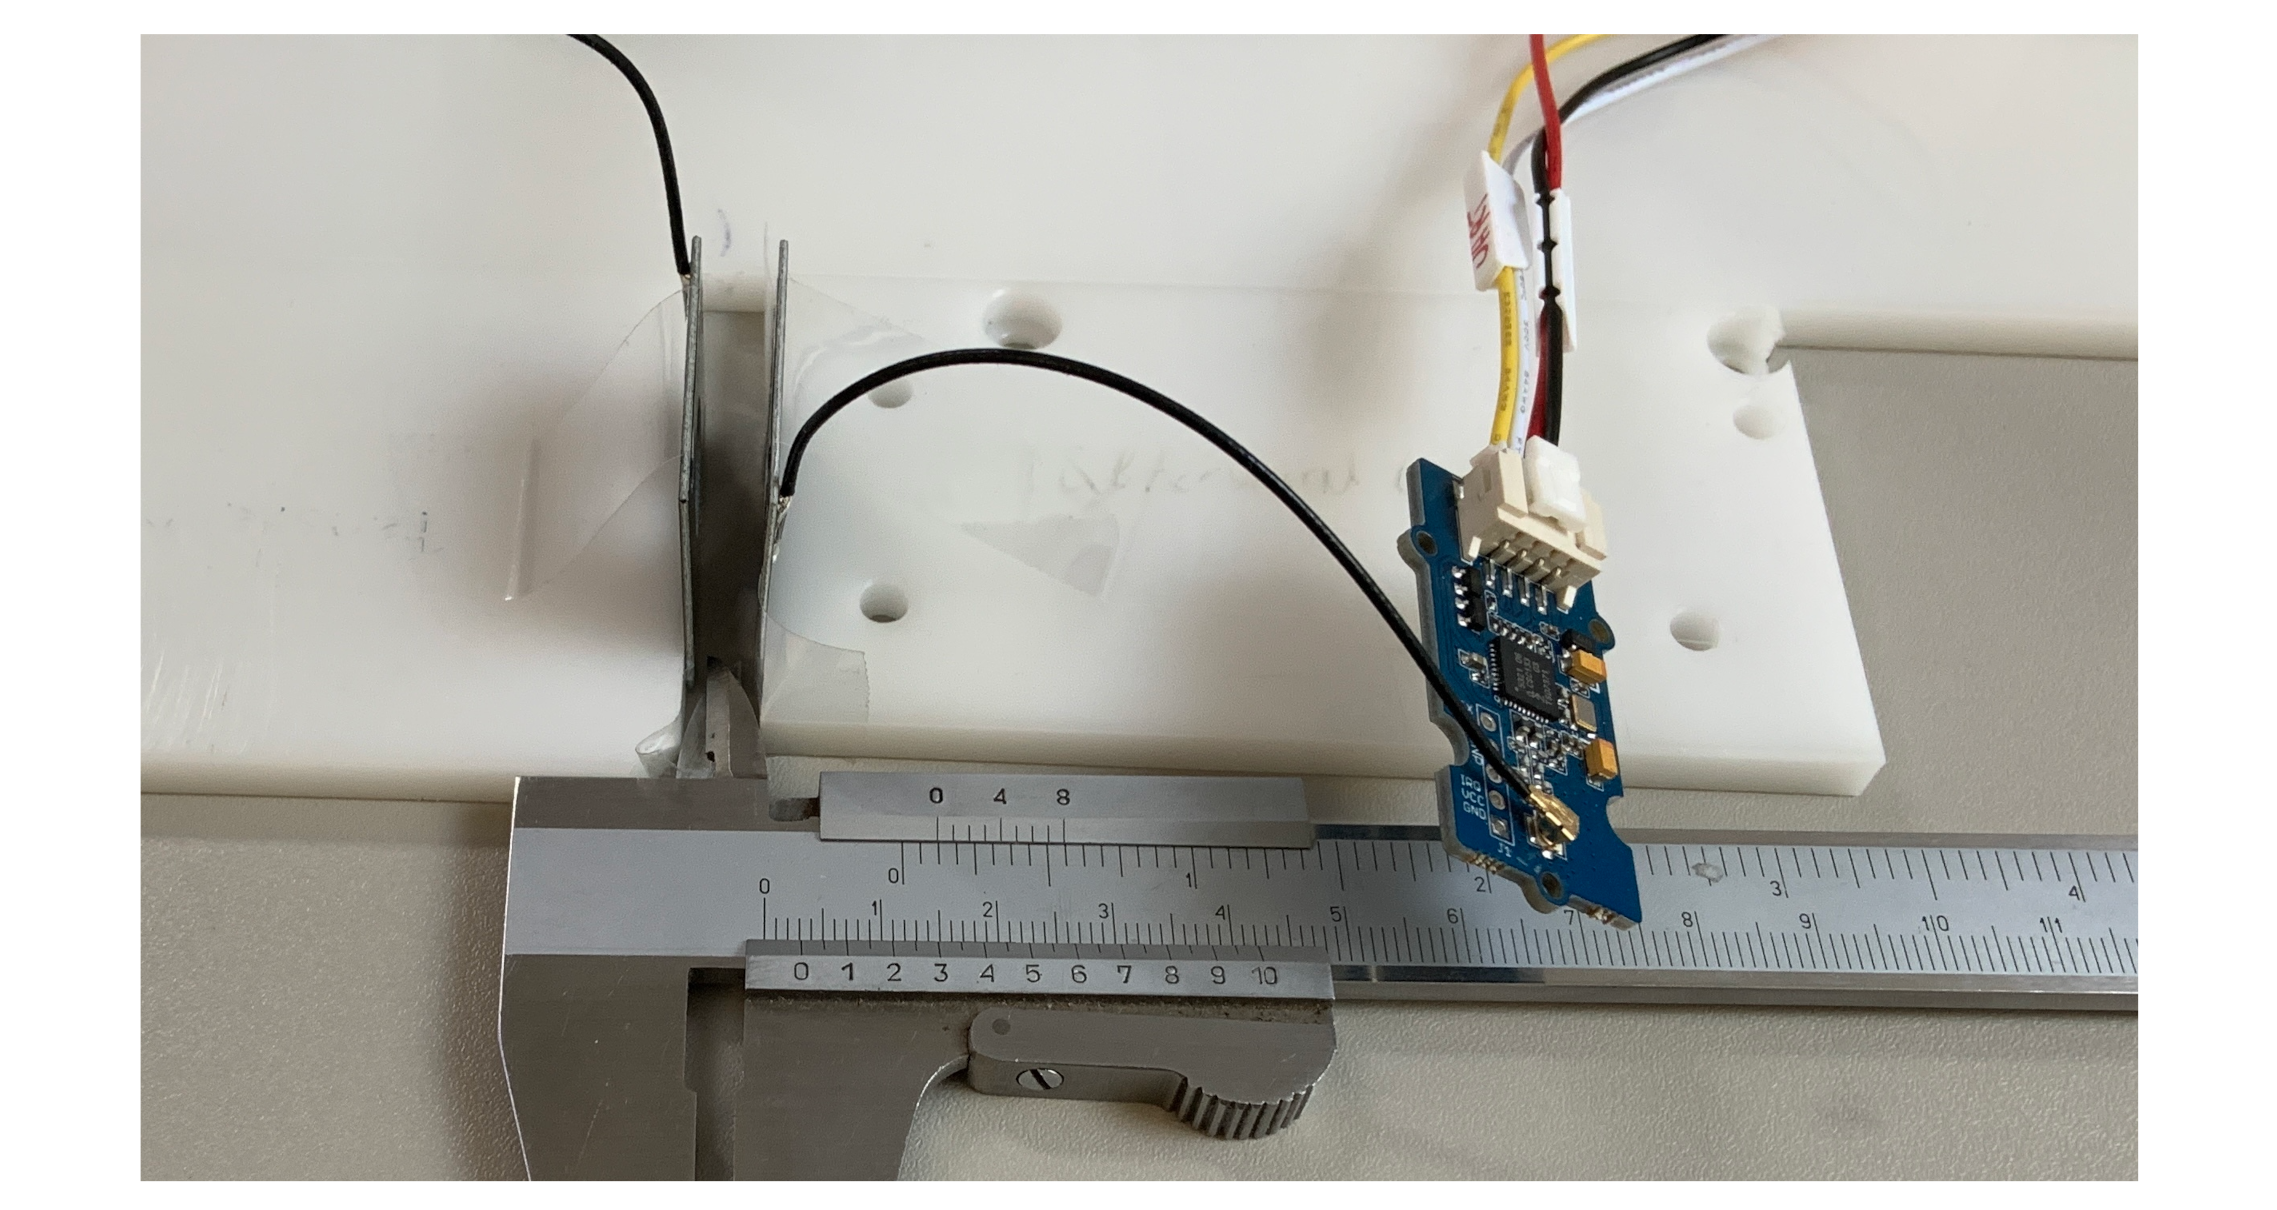
\includegraphics{images/ATC_nfc_range_test.png}
\caption{Grove PN532 NFC Reader mit Kabelgebundener Antenne}
\end{figure}

\begin{itemize}
\tightlist
\item
  test mit figuren nebeneinander
\end{itemize}

\hypertarget{schrittmotor-schrittmotorsteuerung}{%
\subsection{Schrittmotor /
Schrittmotorsteuerung}\label{schrittmotor-schrittmotorsteuerung}}

\begin{itemize}
\tightlist
\item
  warum =\textgreater{} einfache ansteuerung
\item
  keine STEP DIR somit muss embedded nicht echtzeitfähigsein und kann
  ggf auch andere task abbarbeiten
\item
  TMC schrittmotortreiber spi configuration
\item
  und goto move =\textgreater{} wait for move finished irw testen
\item
  dafür einfacher python testreiber geschribene
\item
  schrittverlust nicht zu erwarten
\end{itemize}

\hypertarget{d-druck-fuxfcr-den-mechanischen-aufbau}{%
\subsection{3D Druck für den mechanischen
Aufbau}\label{d-druck-fuxfcr-den-mechanischen-aufbau}}

\begin{itemize}
\tightlist
\item
  PLA als FDM Filament =\textgreater{} einfach verarbeitung und
  handhabung, keine Mechanische Belastbarkeit gefordert
\end{itemize}

Da es sich hier nur um einen Protoypen handelt, wurde hier auf ein
einfach zu handbabendes Filament vom Typ PLA verwendet. Dies ist
besonders gut für die Prototypenendwicklung geeignet und kann mit nahezu
jeden handelsüblichen \gls{fdm} 3D-Drucker verarbeitet werden.

\begin{itemize}
\tightlist
\item
  keine hohe genauigkeit, teile nicht sichtbar
\end{itemize}

Zuvor wurden einige Testdrucke durchgeführt um die Qualität der zuvor
gewählten Druckparameter zu überprüfen und diese gegebenenfalls
anzupassen. Auch wurden verschiedene Calibrierobjekte gedruckt, an
welchen die Toleranzen für die späteren \gls{cad} Zeichnungen abgeschätz
werden können.

Dies betrifft vor allem die Genuigkeit der Bohrungen in den gefertigten
Objekten, da hier später Bolzen und Schrauben ein nahezu spielfrei
eingeführt werden müssen. Ein Test, welcher die Machbarkeit von Gewinden
zeigt wurde nicht durchgeführt, da alle Schrauben später mit der
passenden Mutter gesichert werden sollen. So soll eine Abnutzung durch
häufige Montage der gedruckten Bauteile verhindert werden.

Bei dem Design der zu druckenden Bauteile wurde darauf geachtet, dass
diese den Bauraum von 200x200x200mm nicht überschreiten und somit auch
von einfachen \gls{fdm} 3D-Druckern verarbeitet werden können.

Als Software wurde der Open-Source Slicer Ultimaker Cura
\cite{ultimakercura} verwendet, da dieser zum einen bereits fertige
Konfigurationen für den verwendeten 3D-Drucker enhält und zum anderen
experimentelle Features bereitstellt.

\begin{figure}
\centering
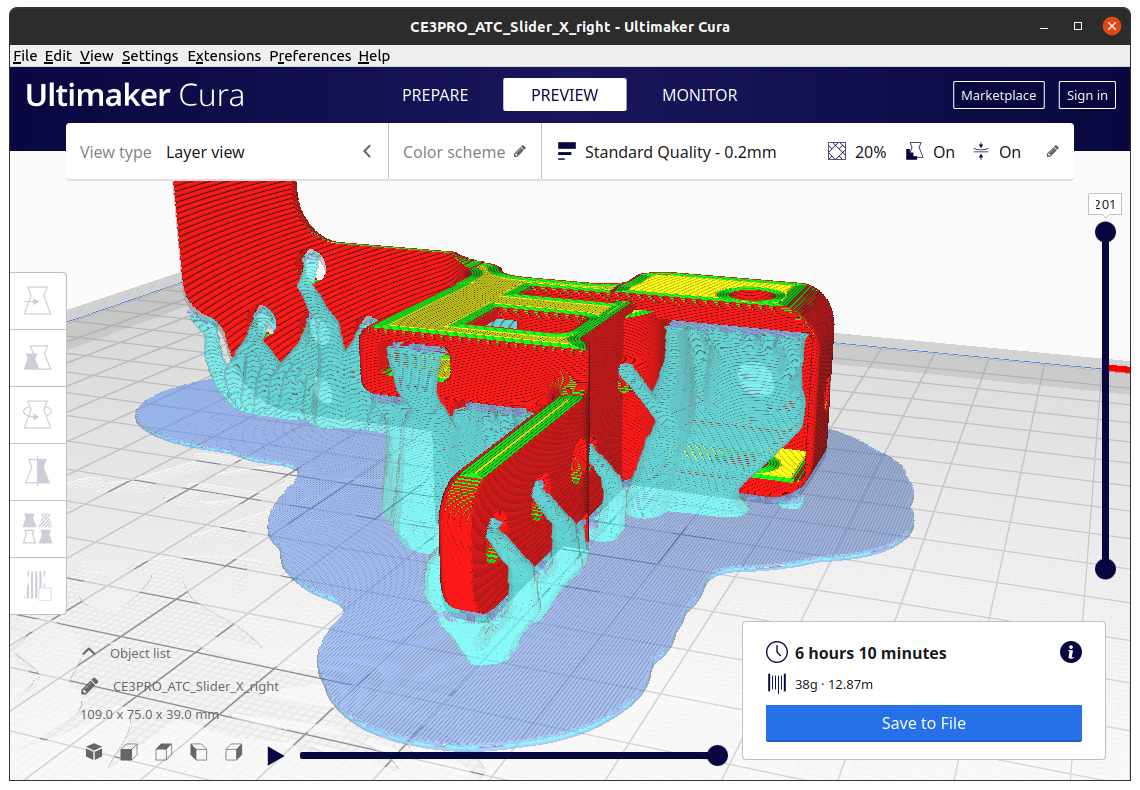
\includegraphics{images/3d_print_tree_structure.png}
\caption{3D Druck: Objekt (rot,gelb,grün),Tree Structure (cyan)}
\end{figure}

Hier wurde für die Bauteile, welche eine Sützstruktur benötigen, die von
Cura bereitgestellte Tree Support Structure aktiviert. Diese bietet den
Vorteil gegenüber anderen Stützstruktiren, dass sich diese leichter
entfernen lässt und weniger Rückstände an den Bauteilen hinterlässt.
Diese Vorteile wurde mit verschiedenen Testdrucken verifiziert und
kommen insbesondere bei komplexen Bauteilen mit innenliegenden Elementen
zum tragen bei denen eine Stützstruktur erfoderlich sind.

\begin{longtable}[]{@{}ll@{}}
\caption{Verwendete 3D Druck Parameter. Temperatur nach
Herstellerangaben des verwendeten PLA Filaments.}\tabularnewline
\toprule
Ender 3 Pro 0.4mm Nozzle & PLA Settings\tabularnewline
\midrule
\endfirsthead
\toprule
Ender 3 Pro 0.4mm Nozzle & PLA Settings\tabularnewline
\midrule
\endhead
Layer Height & 0.2mm\tabularnewline
Infill & 50.00\%\tabularnewline
Wall Thickness & 2.0mm\tabularnewline
Support Structure & Tree\tabularnewline
Top Layers & 4\tabularnewline
Bottom Layers & 4\tabularnewline
\bottomrule
\end{longtable}

\begin{itemize}
\tightlist
\item
  Zeit für den 3D Druck Prozess spiel hier keine Rolle, da selbstbau
  projekt
\item
  Parameter lassen sich weiter anpassen z.B. Layerheight auf 0.4
\item
  finaler protoyp bietet sich abs oder pteg an
\end{itemize}

\hypertarget{erstellung-erster-prototyp}{%
\section{Erstellung erster Prototyp}\label{erstellung-erster-prototyp}}

\begin{itemize}
\item
  proof of conzept
\item
\end{itemize}

\begin{figure}
\centering
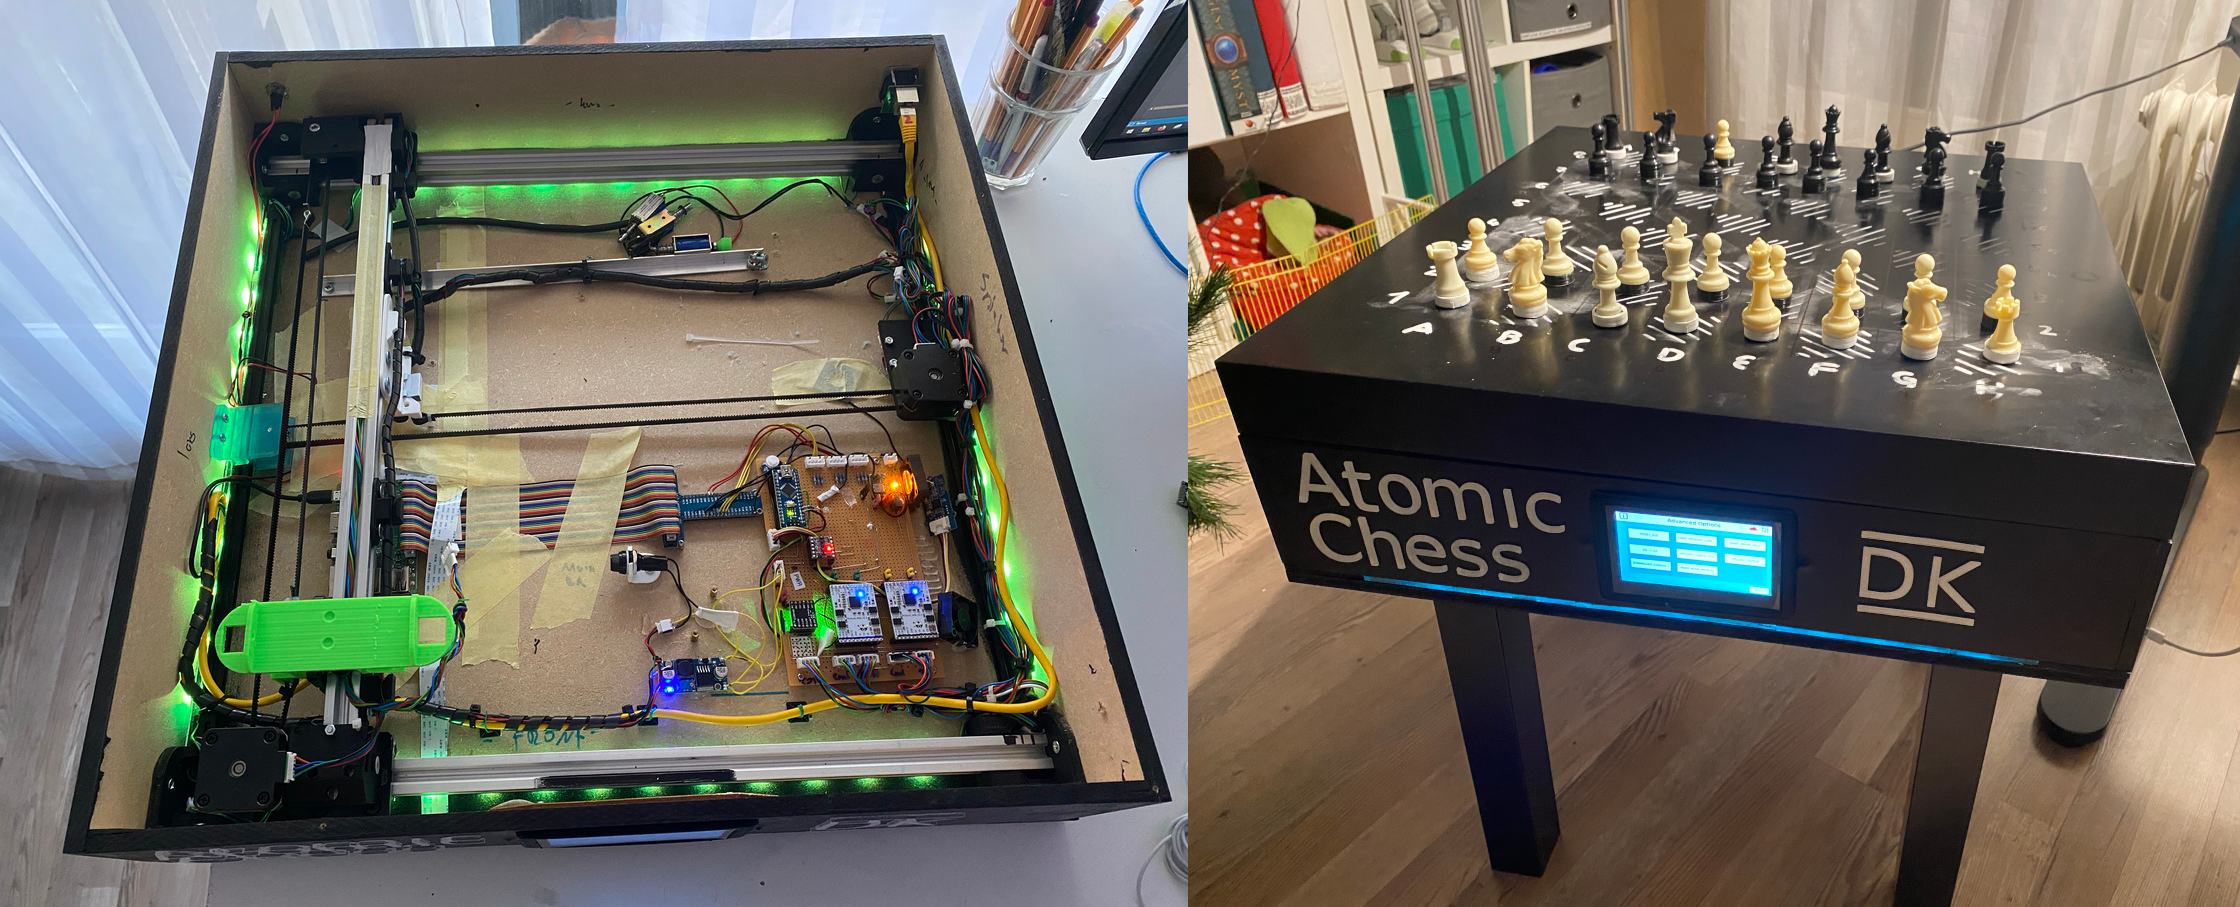
\includegraphics{images/table_images/dk.png}
\caption{Prototyp Hardware: Erster Prototyp des autonomen Schachtisch}
\end{figure}

\hypertarget{mechanik}{%
\subsection{Mechanik}\label{mechanik}}

\begin{itemize}
\item
  vorgaben IKEA tisch als grundbasis =\textgreater{} bereits fertiger
  grundrahmen in denen die einzelteile integriert werden können
\item
  xy riemen führung
\item
  spiel in Mechanik
\item
  Einabrietung in Fusion360
\item
  Cad design aller bauteile
\item
  standartxy
\item
  erweituerng des spielraums durch zwei Magnete
\end{itemize}

\hypertarget{parametrisierung-schachfiguren}{%
\subsection{Parametrisierung
Schachfiguren}\label{parametrisierung-schachfiguren}}

Da das System die auf dem Feld befindlichen Schachfiguren anhand von
\gls{nfc} Tags erkennt, müssen diese zuerst mit Daten beschrieben
werden. Die verwendeten NXP NTAG 21 Chips, besitzen einen vom Benutzer
verwendbaren Speicher von 180 Byte. Dieser kann über ein
\gls{nfc}-Lese/Schreibger mit Daten verschiednster Art beschrieben und
wieder ausgelesen werden. Moderne Mobiltelefone besitzen in der Regel
auch die Fähigkeit mit passenden \gls{nfc} Tags kommunizieren zu können;
somit sind keine Stand-Alone Lesegeräte mehr notwendig.

Der Schachtisch verwendet dabei das \gls{ndef} Dateiformat welches
Festlegt, wie die Daten auf dem \gls{nfc} Tag gespeichert werden. Da
diesen ein Standatisiertes Format ist, können alle gängigen Lesegeräte
und Chipsätze diese Datensätze lesen. Der im autonomen Schachtisch
verwendete Chipsatz PN532 von NXP ist dazu ebenfalls in der Lage.

Um das \gls{ndef} Format verwenden zu können, müssen die \gls{nfc} Tags
zuerst auf diese Formatiert werden. Die mesten käuflichen Tags sind
bereits derart formatiert. Alternativ kann dies mittels Mobiltelefon und
passender App geschehen. Da \gls{ndef} Informationen über die
Formatierung und der gepeicherten Einträge speichert, stehen nach der
Formatierung nur noch 137 Bytes des NXP NTAG 21 zur verfügung.

Per Lesegerät können anschliessend mehrere \gls{ndef} Records auf den
Tag geschrieben werden. Diese sind mit Dateien auf einer Festplatte
vergleichbar und können verschiedenen Dateiformate und Dateigrössen
annehmen. Ein typischer Anwendungsfall ist der \gls{ndefrtd} URL
Datensatz. Dieser kann dazu genutzt werden eine spezifizierte URL auf
dem Endgeräte aufzurufen, nachdem der \gls{nfc} Tag gescant
wurde.\cite{nordicnfclibndef}

Der autonome Schachtisch verwendet den einfachsten \gls{ndefrtd} Typ,
welcher der Text-Record ist, und zum speichern von Zeichenketten genutzt
werden kann, ohne das eine Aktion auf dem Endgerät ausgeführt wird.
Jeder Tag einer Schafigur, welche für den autonomen Schachtisch
verwendet werden kann, besitzt diesen \gls{ndef} Record an der ersten
Position. Alle weiteren eventuell vorhandenen Records werden vom Tisch
ignoriert.\cite{nordicnfclib}

\begin{figure}
\centering
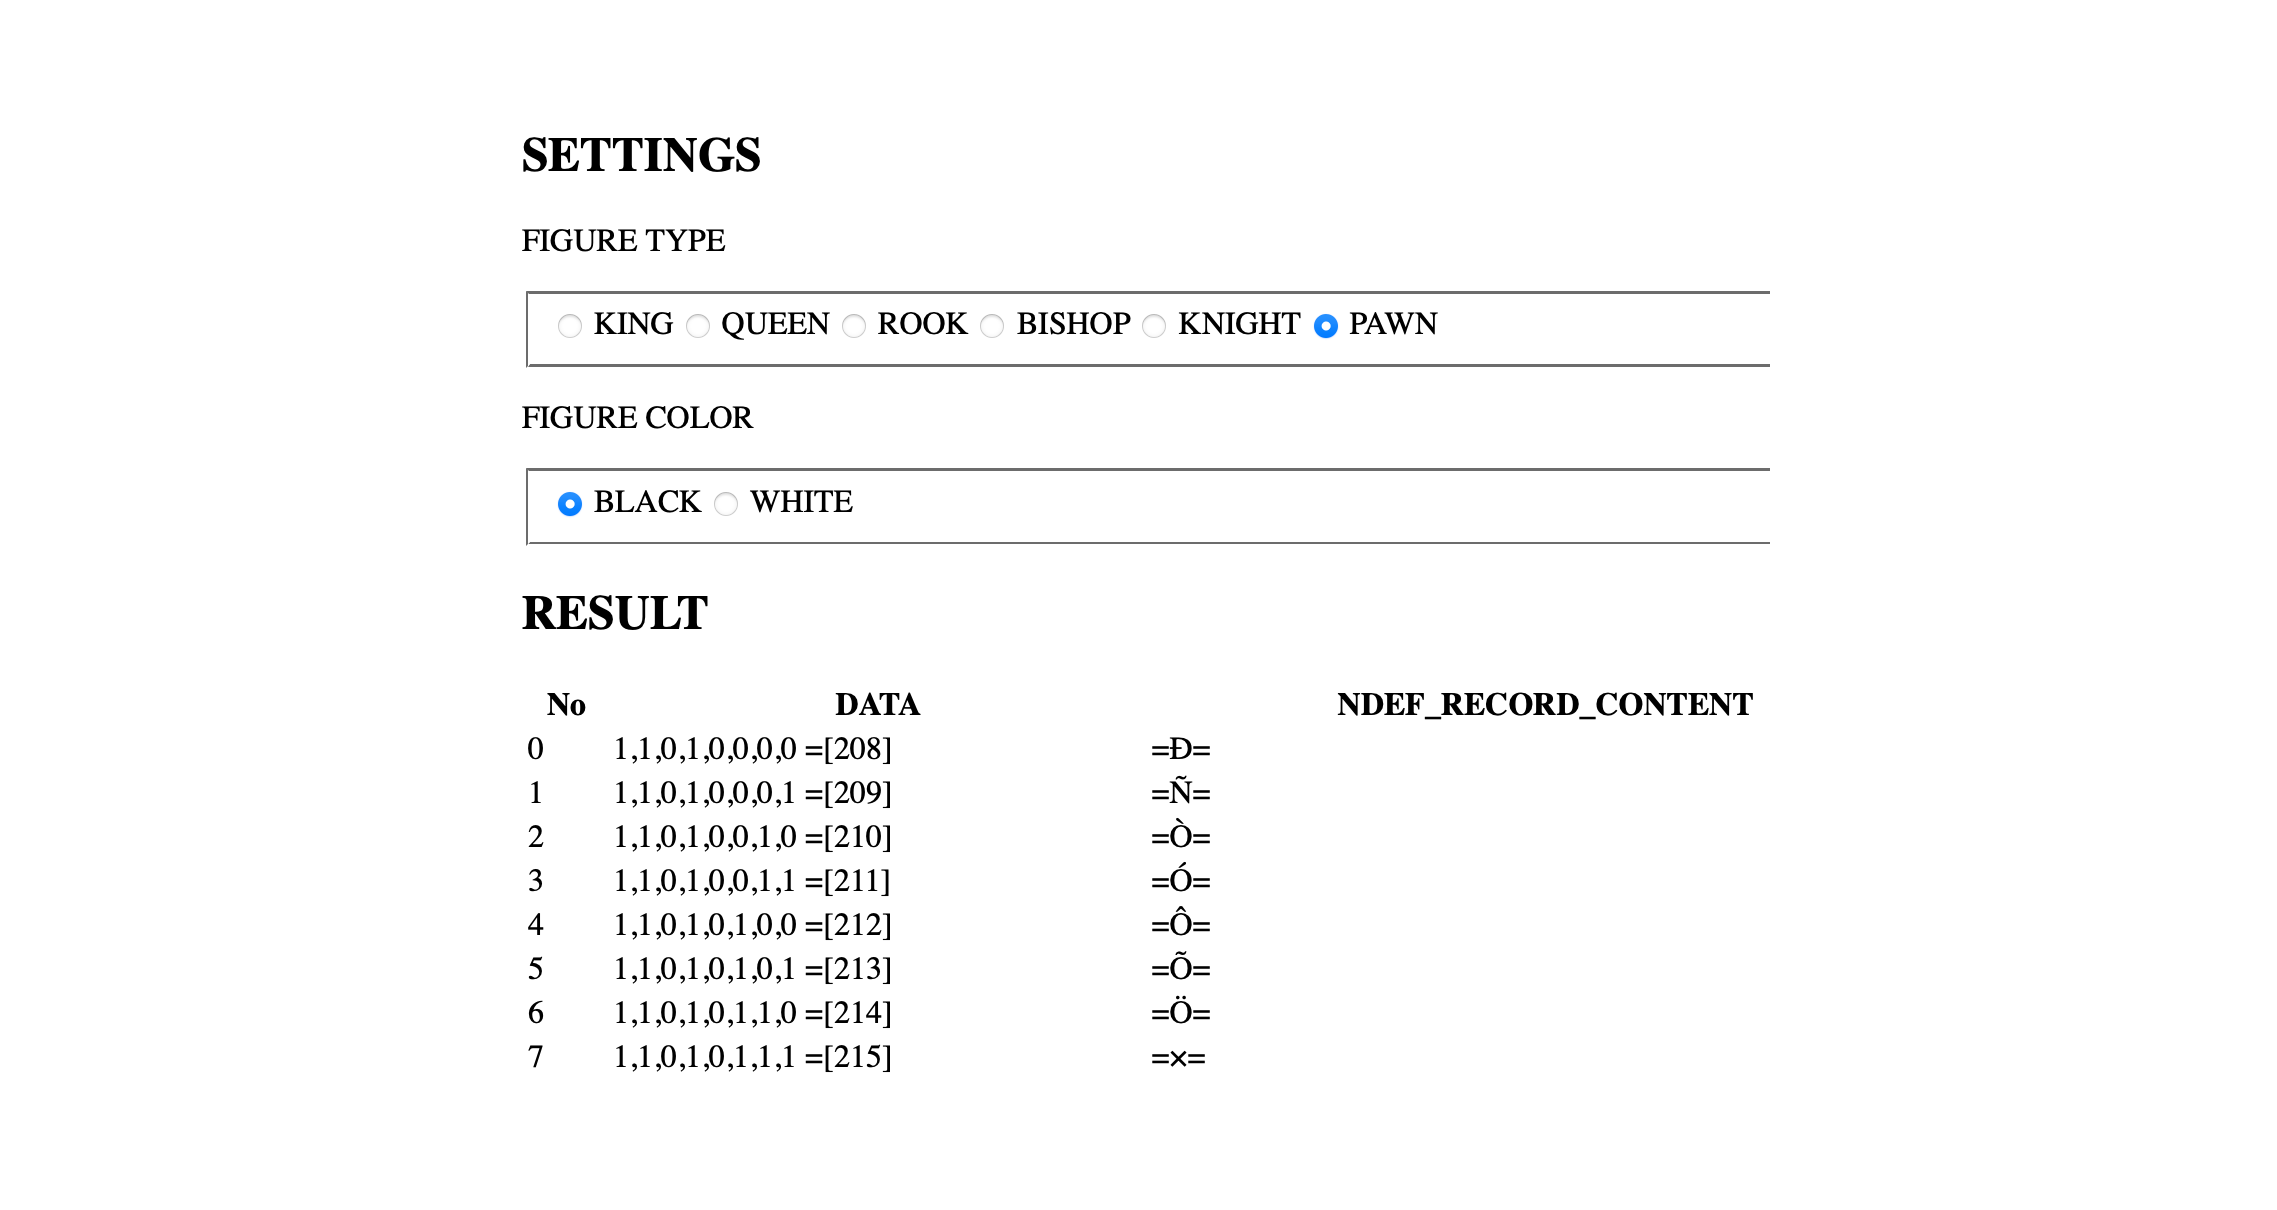
\includegraphics{images/ATC_ChessFigureIDGenerator.png}
\caption{Prototyp Hardware: Tool zur Erstellung des NDEF Payloads:
ChessFigureIDGenerator.html}
\end{figure}

Um die Payload für den \gls{nfc} Record zu erstellen wurde ein kleine
Web-Applikation erstellt, welche den Inhalt der Text-Records erstellt.
Dieser ist für jede Figur individuell und enthält den Figur-Typ und die
Figur-Farbe. Das Tool untersützt auch das Speichern weiterer Attribute
wie einem Figur-Index, welcher aber in der finalen Software-Version
nicht genutzt wird.

Nach dem Beschreiben eines \gls{nfc} Tags ist es möglich diesen gegen
auslesen oder erneuten Schreiben mittels einer Read/Write-Protection zu
schützen. Diese Funktionalität wird nicht verwendet um das Kopieren von
Figuren durch den Benutzer zu ermöglichen. Somit kann dieser leicht
seine eigenen Figuren erschaffen, ohne auf das Tool angewiesen zu sein.
Auch ist es möglich verschiedene Figur-Sets zu mischen, so kann jeder
Spieler sein eigenes Set an Figuren mit dem autonomen Schachtisch
verwenden.

\begin{figure}
\centering
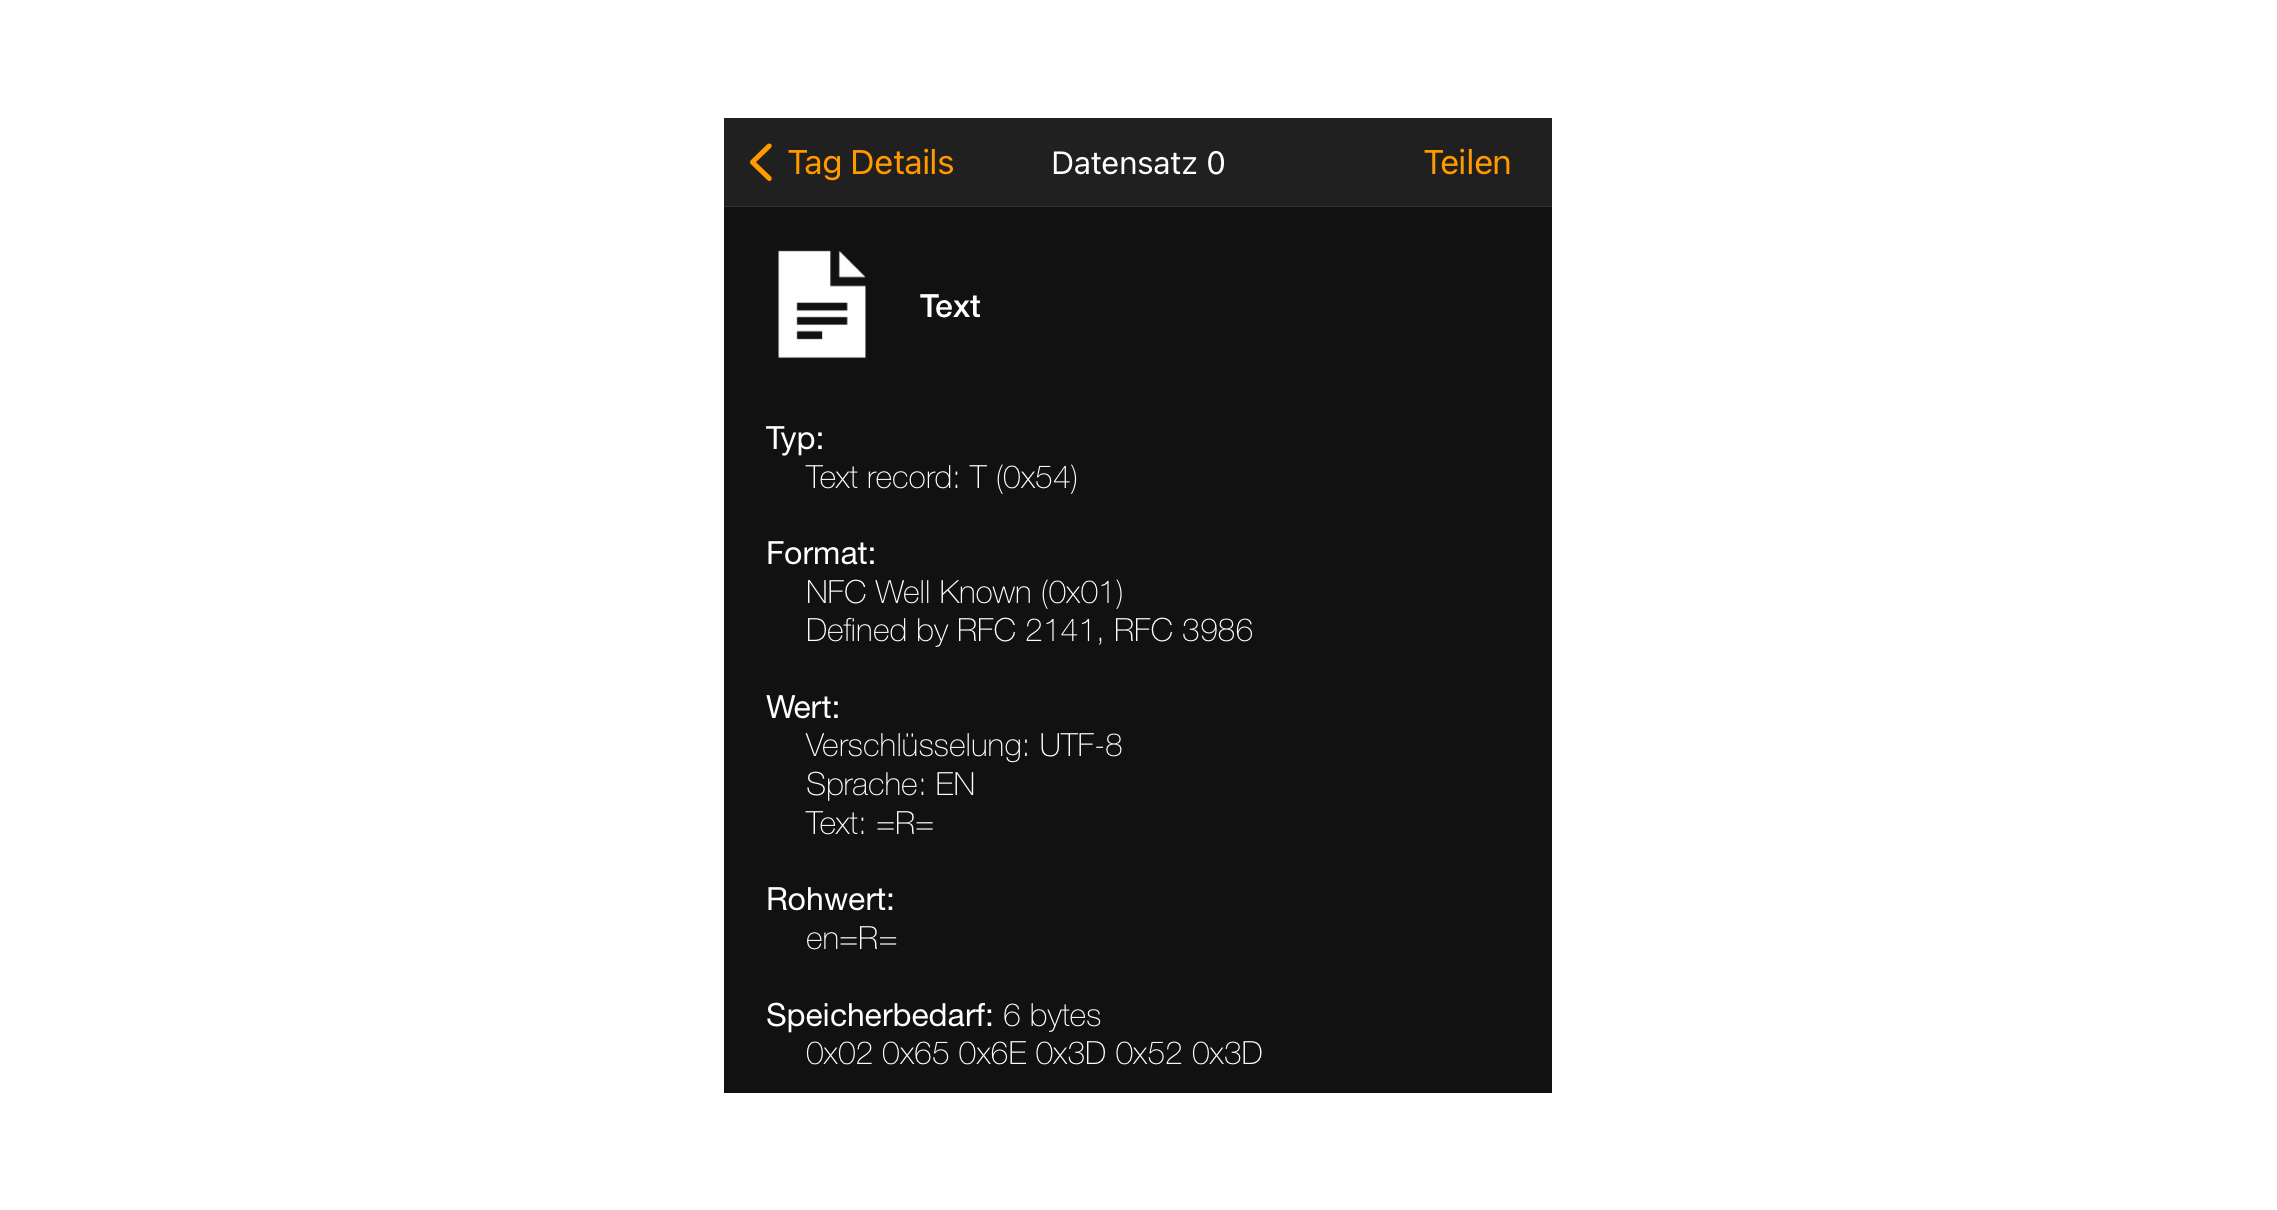
\includegraphics{images/ndef_record_rook.png}
\caption{Prototyp Hardware: NDEF Text Record Payload für einen weissen
Turm}
\end{figure}

\hypertarget{schaltungsentwurf}{%
\subsection{Schaltungsentwurf}\label{schaltungsentwurf}}

\begin{figure}
\centering
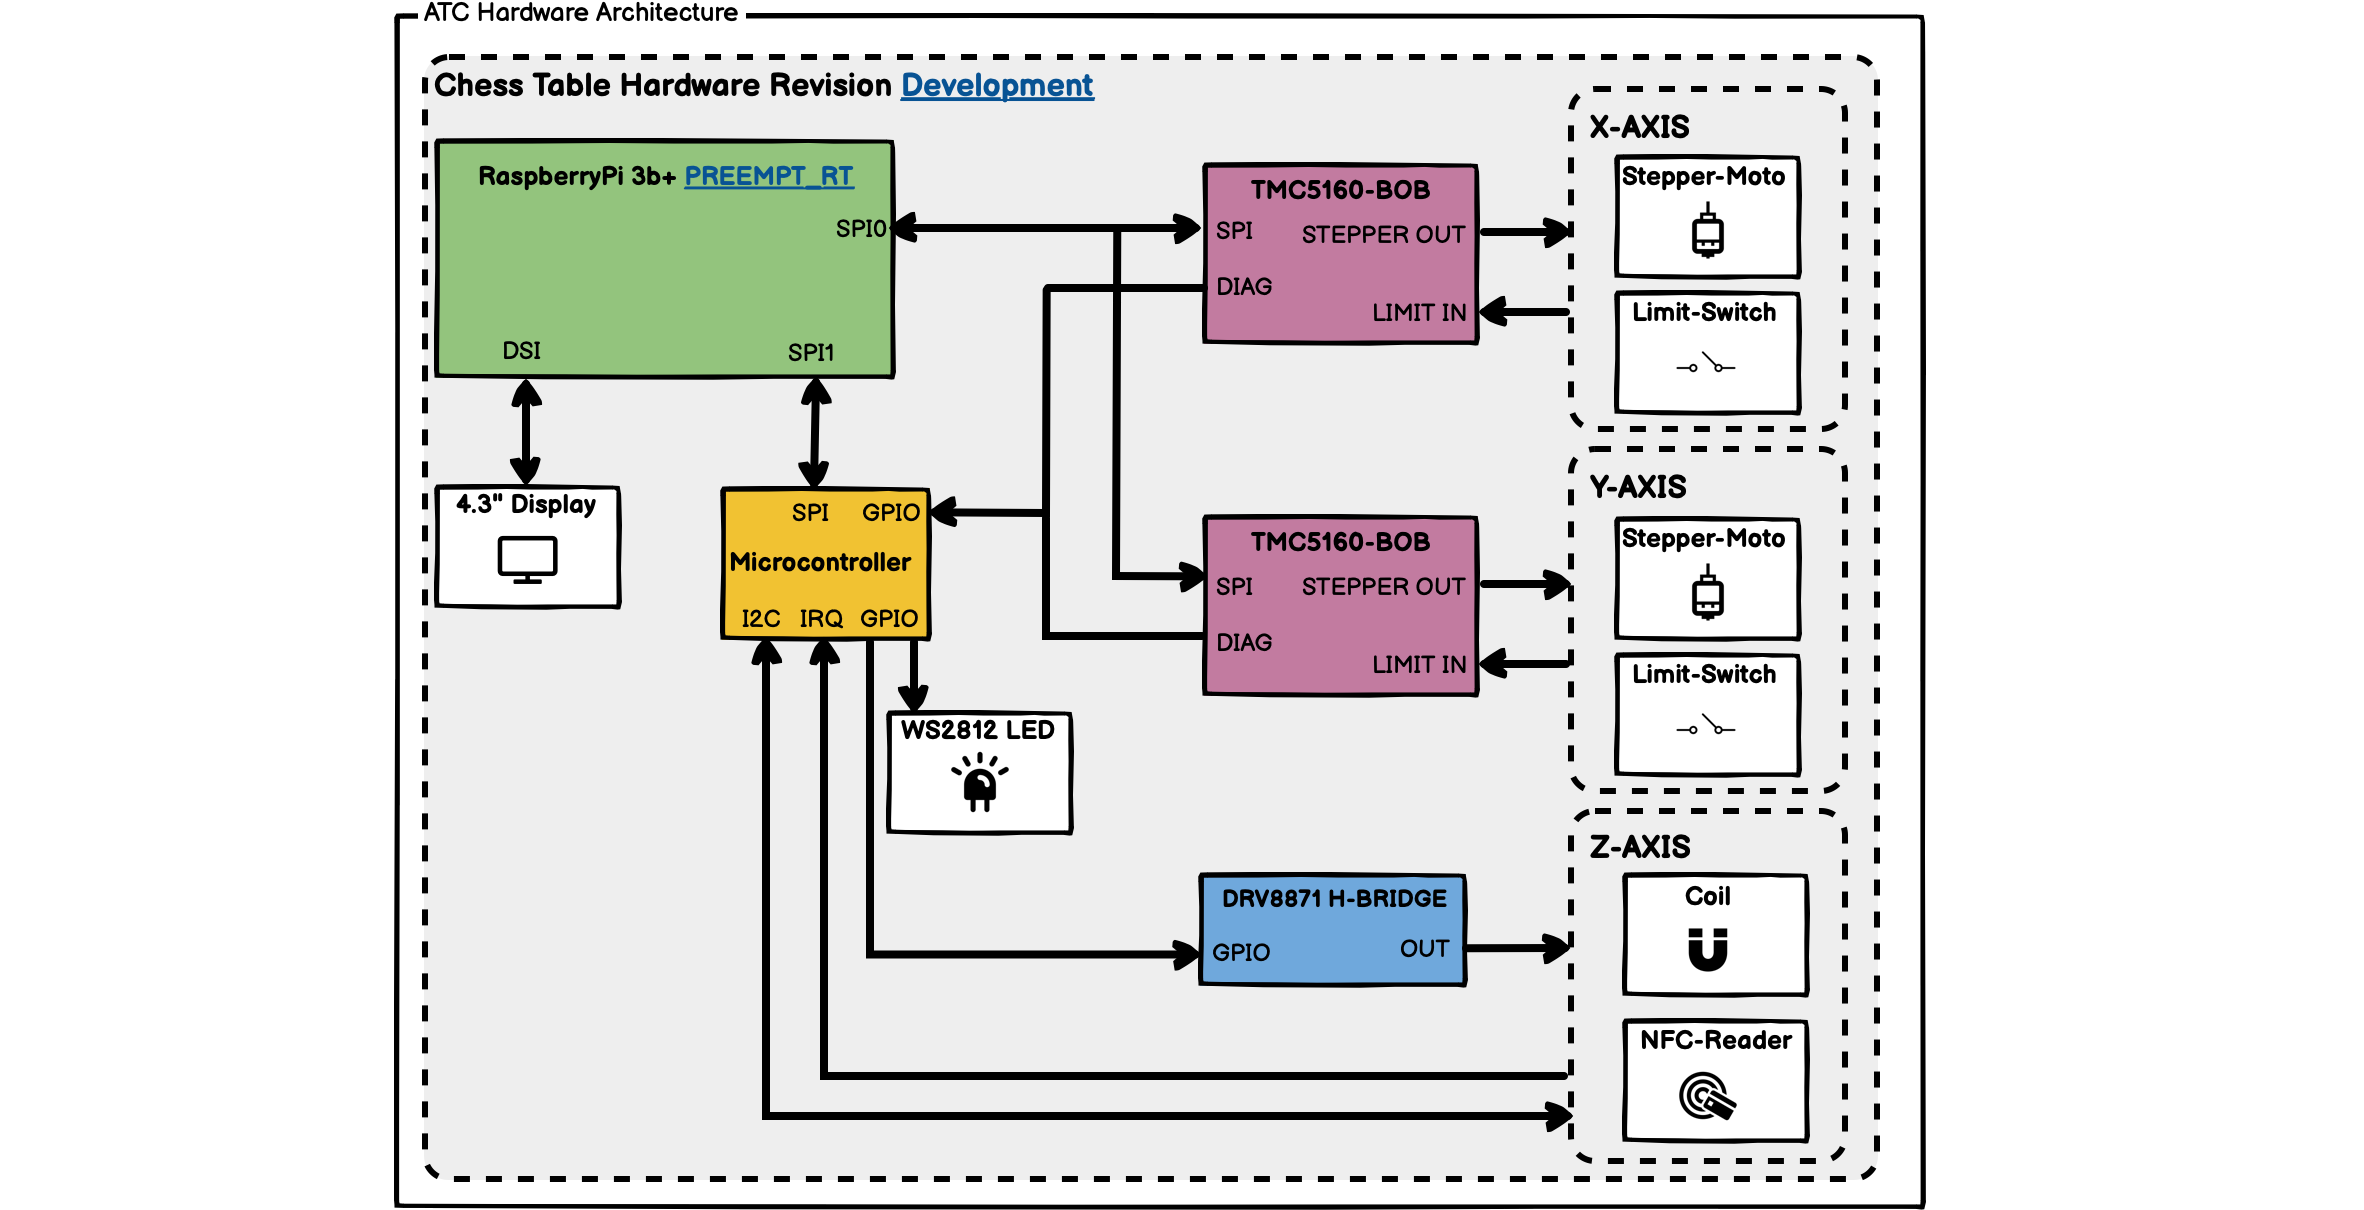
\includegraphics{images/ATC_Hardware_Architecture_DK.png}
\caption{Prototyp Hardware: Blockdiagramm}
\end{figure}

\begin{itemize}
\tightlist
\item
  auswahl der Motortreiber (leise, bus ansteuerung)
\item
  ansteuerung pn532 und umsetzung auf uart
\item
  platinendesign
\item
  ansterung elektromagnetet
\end{itemize}

\hypertarget{implementierung-hal}{%
\subsubsection{Implementierung HAL}\label{implementierung-hal}}

\begin{itemize}
\tightlist
\item
  ansteuerung des TMC5160
\item
  ansterung des Microncontollers (PN532, LED)
\item
  integration in controller software
\end{itemize}

\hypertarget{fazit-zum-ersten-prototypen}{%
\subsection{Fazit zum ersten
Prototypen}\label{fazit-zum-ersten-prototypen}}

\begin{itemize}
\tightlist
\item
  nicht für production geeignet
\item
  aufbau und calibrierung langwiehrig
\item
  trotzdem robustes design auf kleinem formfaktor
\item
  verwendeten elektromagnete nicht stark genug, somit über aqusserhalb
  der specs betrieben was zu temeraturproblemen führte
\item
  gewicht der Figuren zu klein bzw magnete zu start
\item
  workarounds in der software nötig durch die beiden magnete
\item
  nicht die beste entscheidung direkt auf grösse zu optimieren
\end{itemize}

\hypertarget{erstellung-zweiter-prototyp}{%
\section{Erstellung zweiter
Prototyp}\label{erstellung-zweiter-prototyp}}

\begin{figure}
\centering
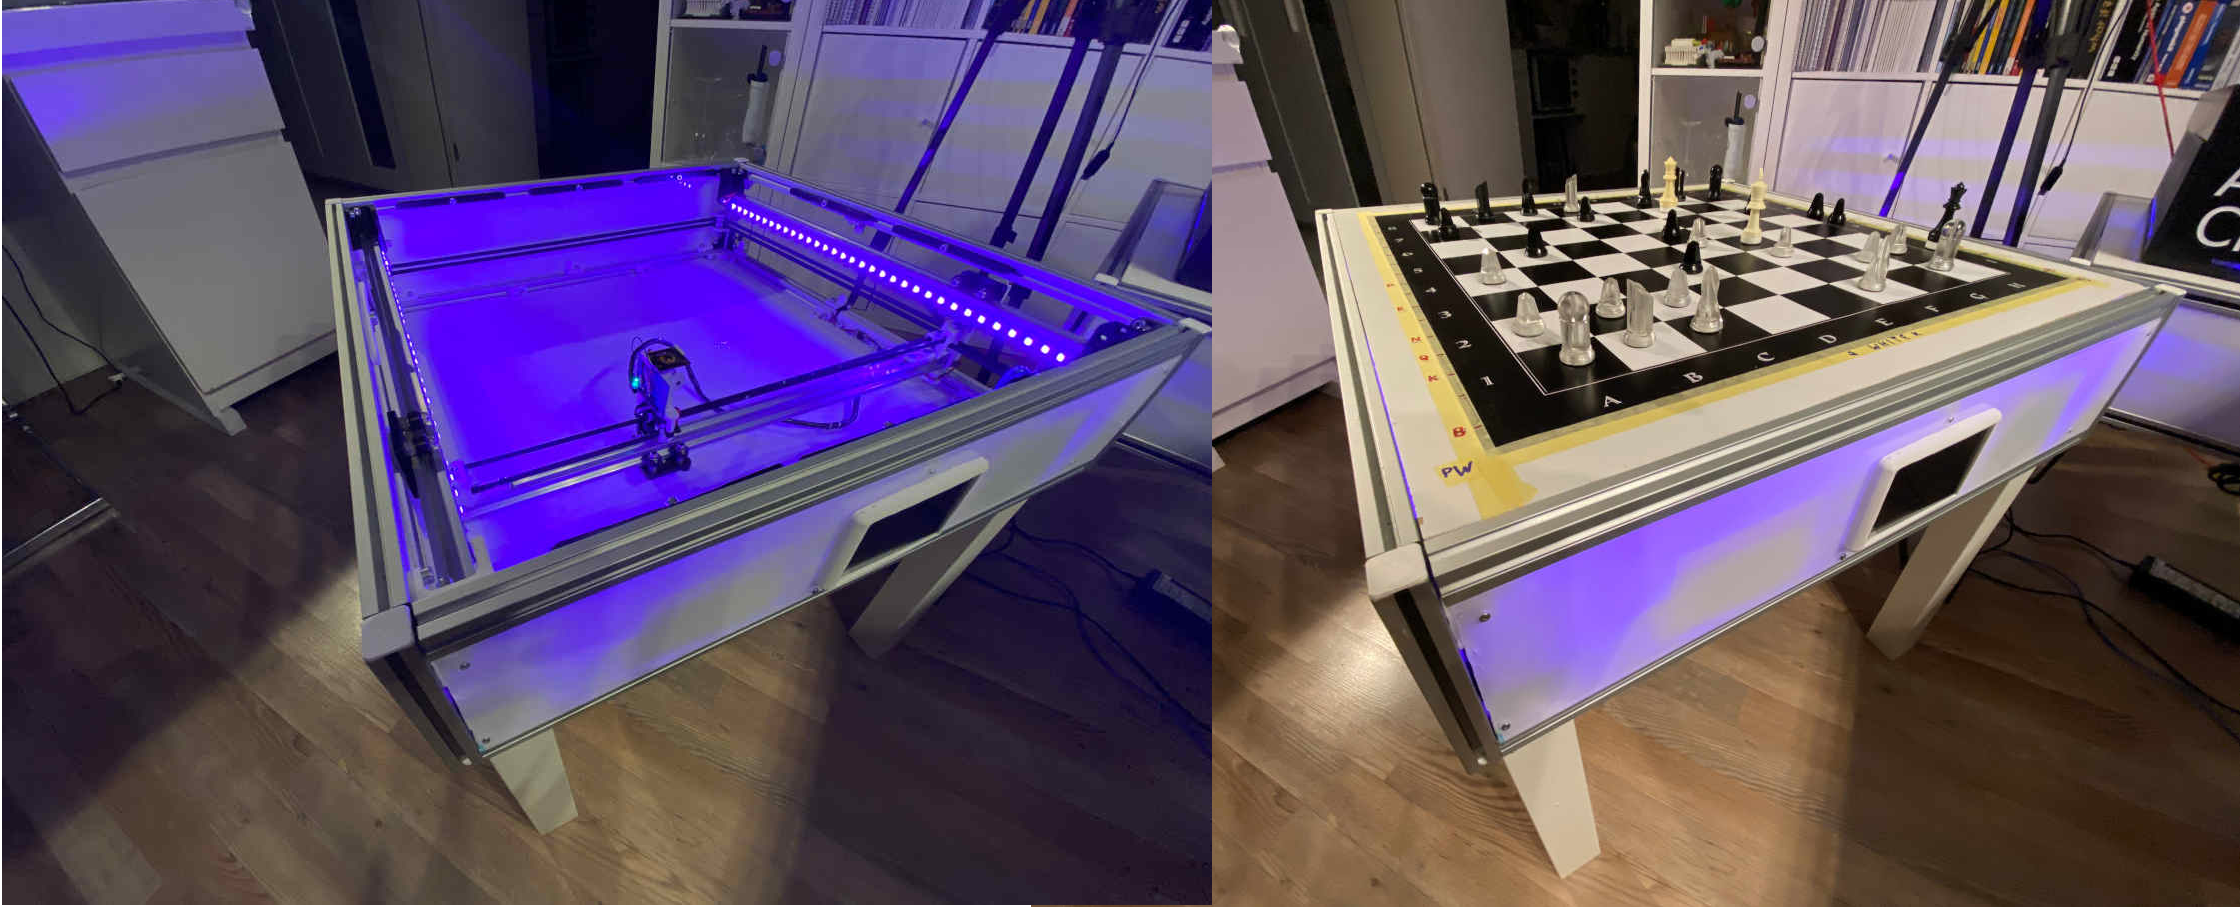
\includegraphics{images/table_images/prod.png}
\caption{Producation Hardware: Finaler autonomer Schachtisch}
\end{figure}

\hypertarget{modifikation-der-mechanik}{%
\section{Modifikation der Mechanik}\label{modifikation-der-mechanik}}

\begin{itemize}
\tightlist
\item
  dauertest hat gezeigt dass mechnik zu viel spiel aufweisst
\item
  Motorenhalterung der y achse schränkt des bewegungsspielraum um mehr
  als 10cm ein, welches zu einem unwesentlichen grösseren verhältnis von
  Spielfeldgrösse und Abmessungen des Schachtischs
\item
  CoreXY bietet Vorteil:
\item
  Motoren fest am rahmen =\textgreater{} weniger kabel + gewicht an der
  Y Achse
\item
  jedoch komplexerer Aufwand der riemenverlegung so komplexere 3d
  bauteile
\item
  Tischabmessungen 620x620mm dabei Bewegungsspielraum vom 580x580 zuvor
  nur 480x480
\end{itemize}

\hypertarget{optimierungen-der-spielfiguren}{%
\section{Optimierungen der
Spielfiguren}\label{optimierungen-der-spielfiguren}}

Die bisherigen genutzen vorgefertigten Figuren funktionierten mit dem
ersten Prototyp problemlos. Sie wiesen aber trotzdem eine zu hohe
Fehleranfälligkeit, im Bezug auf das gegenseitige Beeinflussen
(abstoßen,anziehen) durch die verwendeten Magnete.

Die größse der Figuren kann durch die fest definierte Feldgrösse von
55mm und der verwendeten \gls{nfc} Tags nicht verändert werden. Nach
vielen Testdurchläufen mit dem ersten Prototyp war zu erkennen, dass
sich die Figuren je nach aktueller Situation auf dem Spielfeld immernoch
magnetisch anziehen. Dies führt je nach Spielverlauf zu Komplikationen,
sodass die Figuren manuell wieder mittig auf den Felder platziert werden
müssen.

Um dies zu verhindern, wurde einige Figuren zusätzlich mit einer 20mm
Unterlegscheibe am Boden versehen, welche diese Problem behob, jedoch
das \gls{nfc} Tag nicht mehr als lesbar erwies. Dies resultierte in der
Idee die Schachfiguren ebenfalls selbst mit dem 3D-Drucker herzustellen
und die Magnete direkt in den Boden der Figur einlassen zu können.

Die aktuell verwendeten Figuren des ersten Protoyp wiegen 8 Gramm für
die Bauern und 10 Gramm für die restlichen Figuren. Der Test mit der
Unterlegscheibe ergab, dass diese mit 4 Gramm genug Gewicht hinzufügte
um die magnetische Beeinflussung zu unterbinden.

Testweise wurden eingie Figuren mittels 3D Drucker erstellt um so das
Gewicht zu erhöhen. Nach einem erfolgreichen Test wurde das \gls{cad}
Modell wurde so angepasst, dass sich der Magnet direkt in den Boden der
Figure einkleben lässt. Desweiteren wurden bei den Bauern (den
leichtesten) Figuren die Magnete ausgetauscht. Die zuerst verwendeten
10x3mm Neodym-Magnete wurden bei diesen Figuren gegen 6x3mm Magnete
getauscht. Somit sind im Design zwei verschiedenen Arten von Magneten
notwendig, jedoch traten in den anschliessend durchgeführten Testläufen
keine Beeinflussungen mehr statt.

\begin{itemize}
\item
  komplett 3d gedruckte Figuren mit integrierten Magnet
\item
  nfc + filzgleiter
\item
  durch SLA druck höheres Gewicht somit kein Abstoßen von den anderen
  Figuren mehr
\item
  verschiedene Magnetgrässe/Stärke für Bauern/andere Figuren
\item
  jedoch alte figuren weiter verwendbar und austausch / vermischbar
\end{itemize}

\hypertarget{uxe4nderungen-der-elektronik}{%
\section{Änderungen der Elektronik}\label{uxe4nderungen-der-elektronik}}

\begin{figure}
\centering
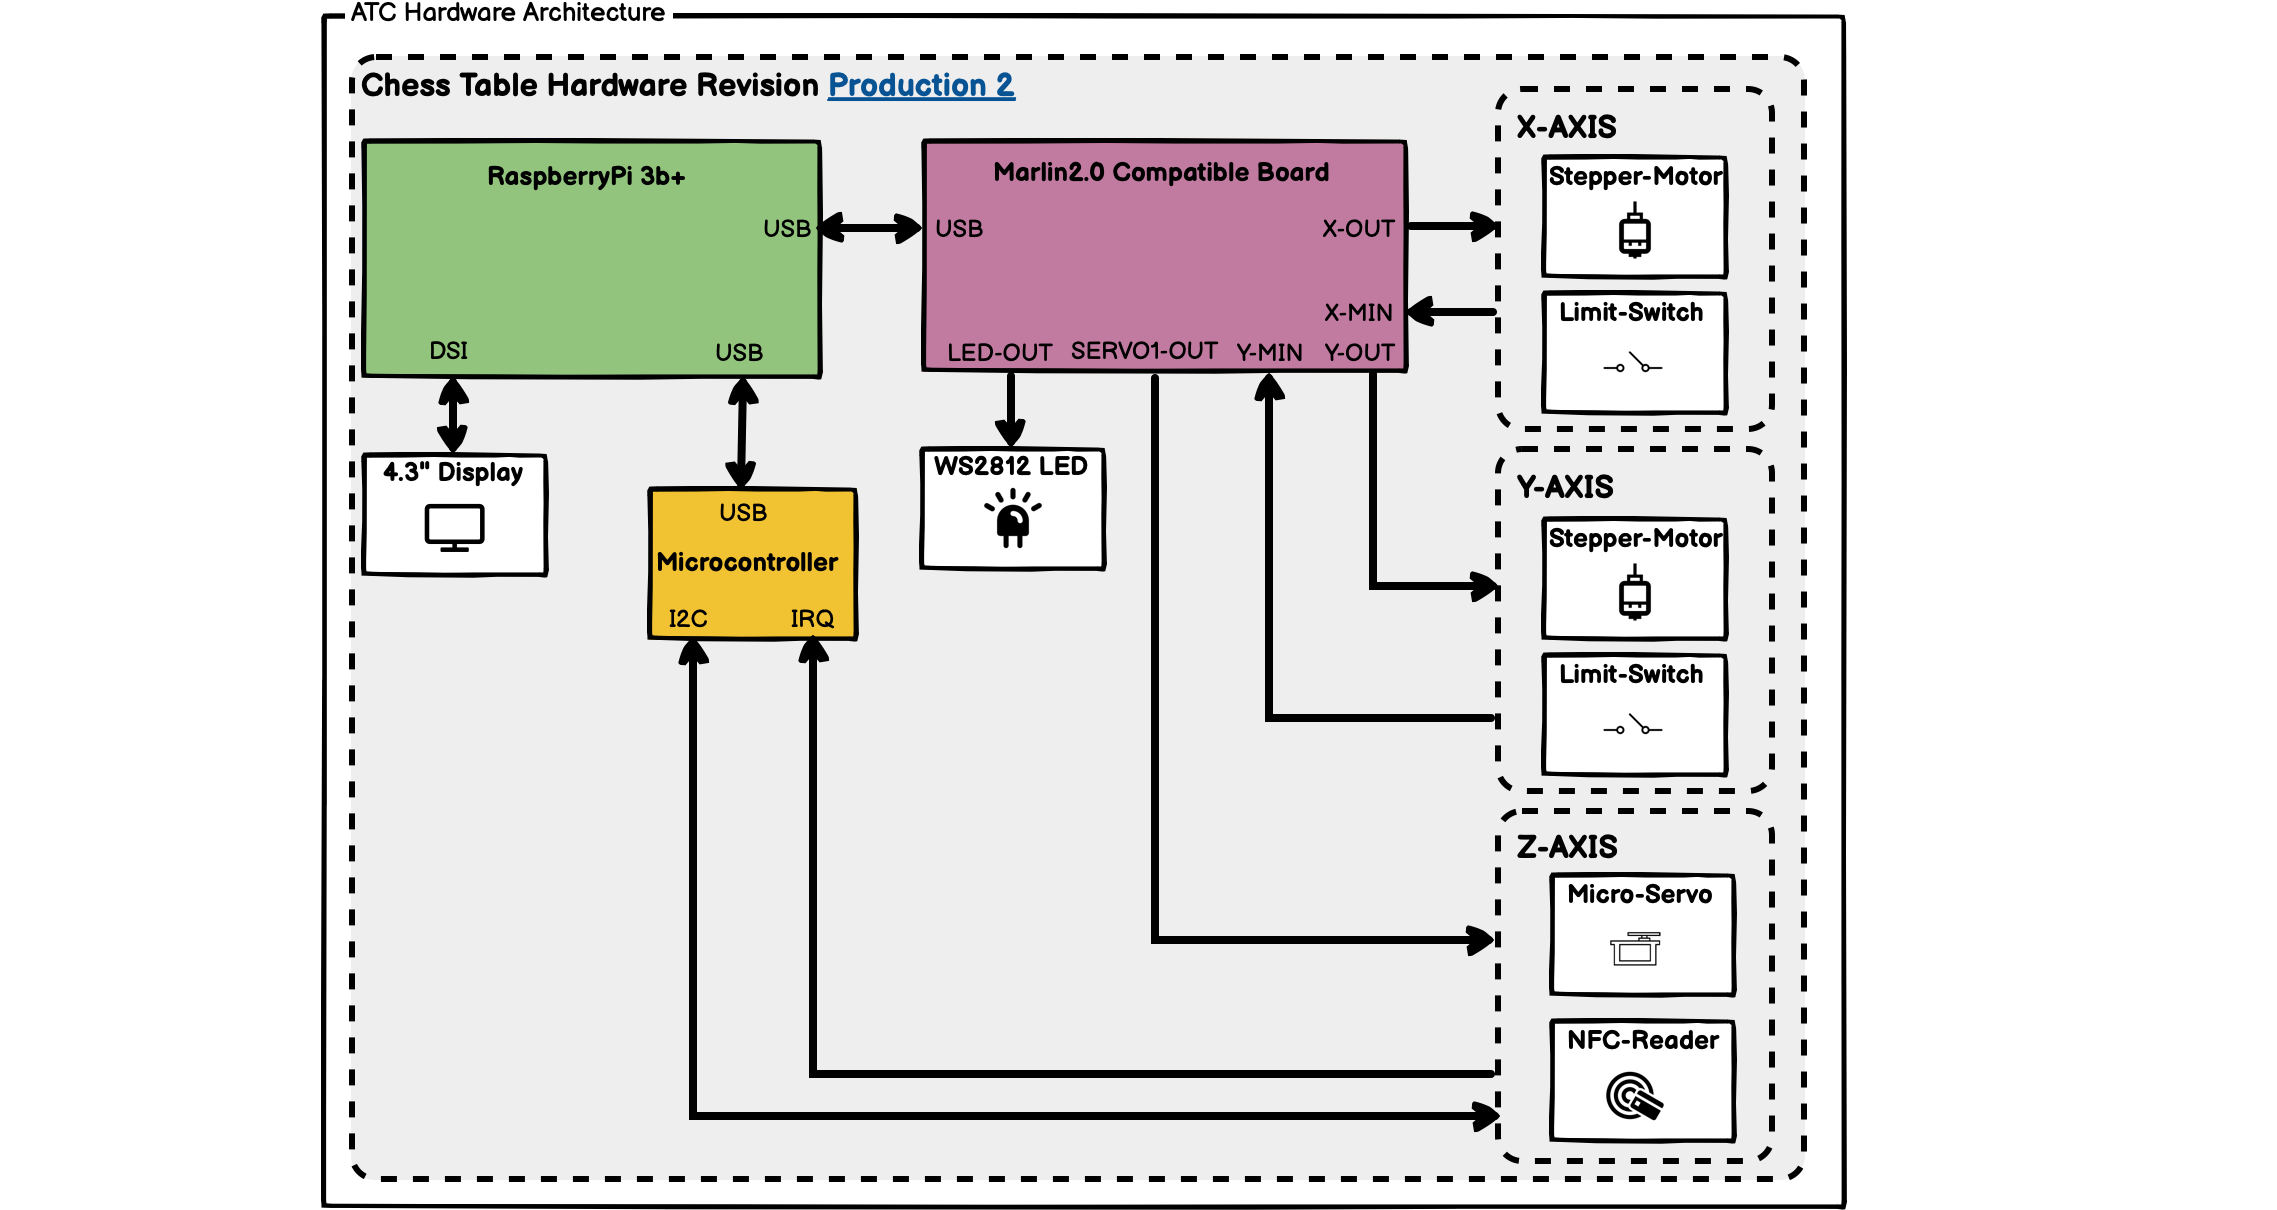
\includegraphics{images/ATC_Hardware_Architecture_PROD.png}
\caption{Producation Hardware: Blockdiagramm}
\end{figure}

\begin{itemize}
\tightlist
\item
  verwenung von standarthardware, welche gut zu beschaffen ist
\item
  implementierung von standart gcode protokol, somit mit universell
  verwendbaren steuerung verwendbar
\item
  bietet eine hohe flexibilität da nur ein minimales set von
  Gcode-kommandos vorrausgesetzt wird
\end{itemize}

\hypertarget{implementierung-gcode-sender}{%
\subsection{IMPLEMENTIERUNG
GCODE-Sender}\label{implementierung-gcode-sender}}

\begin{itemize}
\item
  was ist GCODE
\item
  grundlegend verwendete Kommandos G0 G28 G21 G90 M280
\item
  erweiterte optionale Kommandos M150 M502 M500 M92
\item
  anhand der hwid und existenz der serial interfaces wird entschieden
  gcode hardware zu laden
\item
\end{itemize}

\hypertarget{fazit-zum-finalen-prototypen}{%
\subsection{Fazit zum finalen
Prototypen}\label{fazit-zum-finalen-prototypen}}

\begin{itemize}
\tightlist
\item
  modularer hardware aufbau
\item
  einfach/gut verfügbare materialien verwendet
\item
  geänderte Mechnik resultiert in nahezu Spielfreier Mechanik (+- 1mm),
  welches für diesen Zweck mehr als ausreicht
\item
  6h dauertest bestanden
\end{itemize}

\hypertarget{entwicklung-der-cloud-infrastruktur}{%
\section{Entwicklung der Cloud
Infrastruktur}\label{entwicklung-der-cloud-infrastruktur}}

Die erste Phase der Entwicklung des Systems bestand in der Entwicklung
der Cloud-Infrastruktur und der darauf laufenden Services. Hierbei
stellt die ``Cloud'', einen Server dar, welcher aus dem Internet über
eine feste IPv4 und eine IPv6 verfügt und frei konfiguriert werden kann.

\begin{figure}
\centering
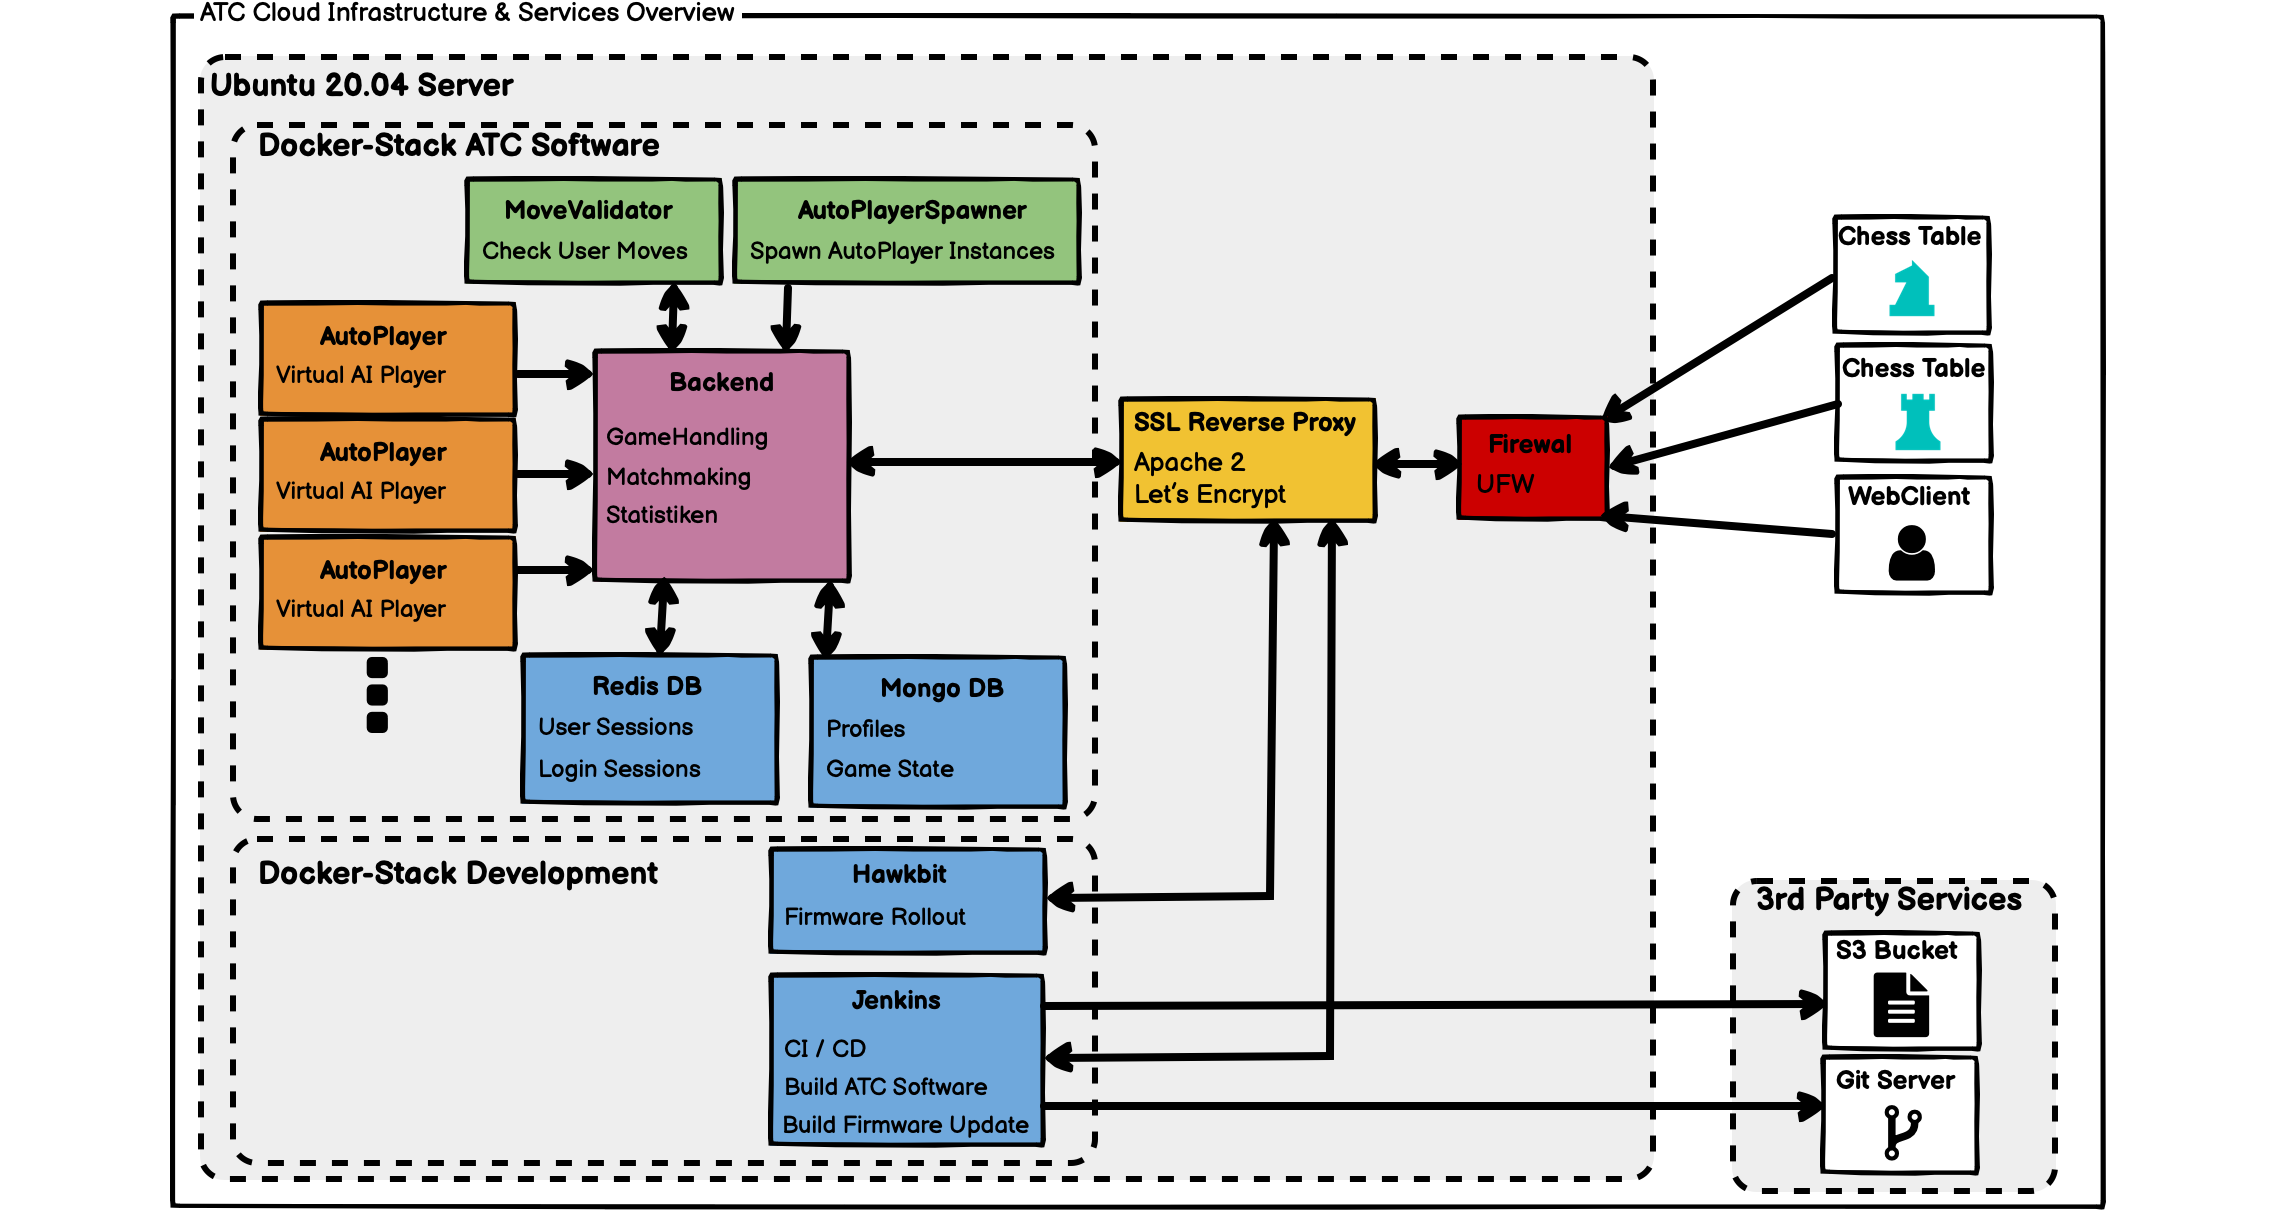
\includegraphics{images/ATC_Cloud_Architecture.png}
\caption{Cloud-Infrastruktur: Gesamtübersicht der verwendeten
Cloud-Infrastruktur}
\end{figure}

\hypertarget{api-design}{%
\subsection{API Design}\label{api-design}}

Das System soll so ausgelegt werden, dass es im späteren Zeitpunkt mit
verschiedenen Client-Devices mit diesem kommunizieren können. Dazu
zählen zum einen der autonome Schachtisch, aber z.B. auch einen
Web-Client, welcher die Funktionalität eines Schachtisch im Browser
abbilden kann. Hierzu muss das System eine einheitliche
\gls{rest}-Schnittstelle bereitstellen.

Eine RESTful API bezeichnet eine API welche HTTP-Requests verwendet um
auf Daten zugreifen zu können.

\begin{itemize}
\tightlist
\item
  grafik
\item
  5 requirements
\end{itemize}

Die RESTful API stellt verschiedene Ressourcen bereit, welche durch eine
URI eindeutig identifizierbar sind. Auf diese können mittels
verschiedenster HTTP Anfragemethoden (GET, POST, PUT, DELETE)
zugegriffen werden. Jeder dieser Methoden stellt einen anderen Zugriff
auf die Ressource dar und beeinflusst somit das Verhalten und die
Rückantwort dieser.

\begin{figure}
\centering
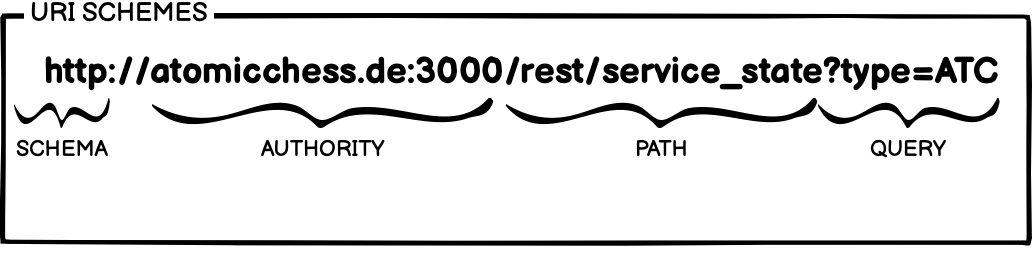
\includegraphics{images/ATC_URI_SCHEMES.png}
\caption{Cloud-Infrastruktur: Aufbau einer URI}
\end{figure}

Eine URI besteht dabei aus mehreren Teilen. Das Schema gibt an wie die
nachfolgenden Teile interpretiert werden sollen. Dabei wird bei einer
RESTful Schnittstelle typischerweise das \gls{http} Protokoll, sowie
\gls{https} verwendet. Dabei steht \gls{https} für eine verschlüsselte
Verbindung. Desweiteren gibt es viele andere Schema, wie z.B \gls{ftp}
welches

Somit stellt die RESTful API eine Interoperabilität zwischen
verschiedenen Anwendungen und Systemen bereit, welche durch ein Netzwerk
miteinander verbunden sind. Dieser Ansatz ist somit geeignet um die
verschiedenen Client Systeme (Schachtisch, Webclient) eine Kommunikation
mit dem Server zu erlauben.

\hypertarget{service-architektur}{%
\subsection{Service Architektur}\label{service-architektur}}

\begin{itemize}
\tightlist
\item
  was ist ein Service
\item
  microservice ansatz
\item
  Kapselung der Schach spiel spzifischen funktionaliutäten
\item
  verwendung von NoSQL Datenbanken somit müssen tabellen nicht spzeill
  auf Schach spezifische felder ausgelegt sein
\item
  statelss Diese stellen alle wichtigen Funktionen zum Betrieb des
  autonomen Schachtischs zur verfügung.
\end{itemize}

\begin{figure}
\centering
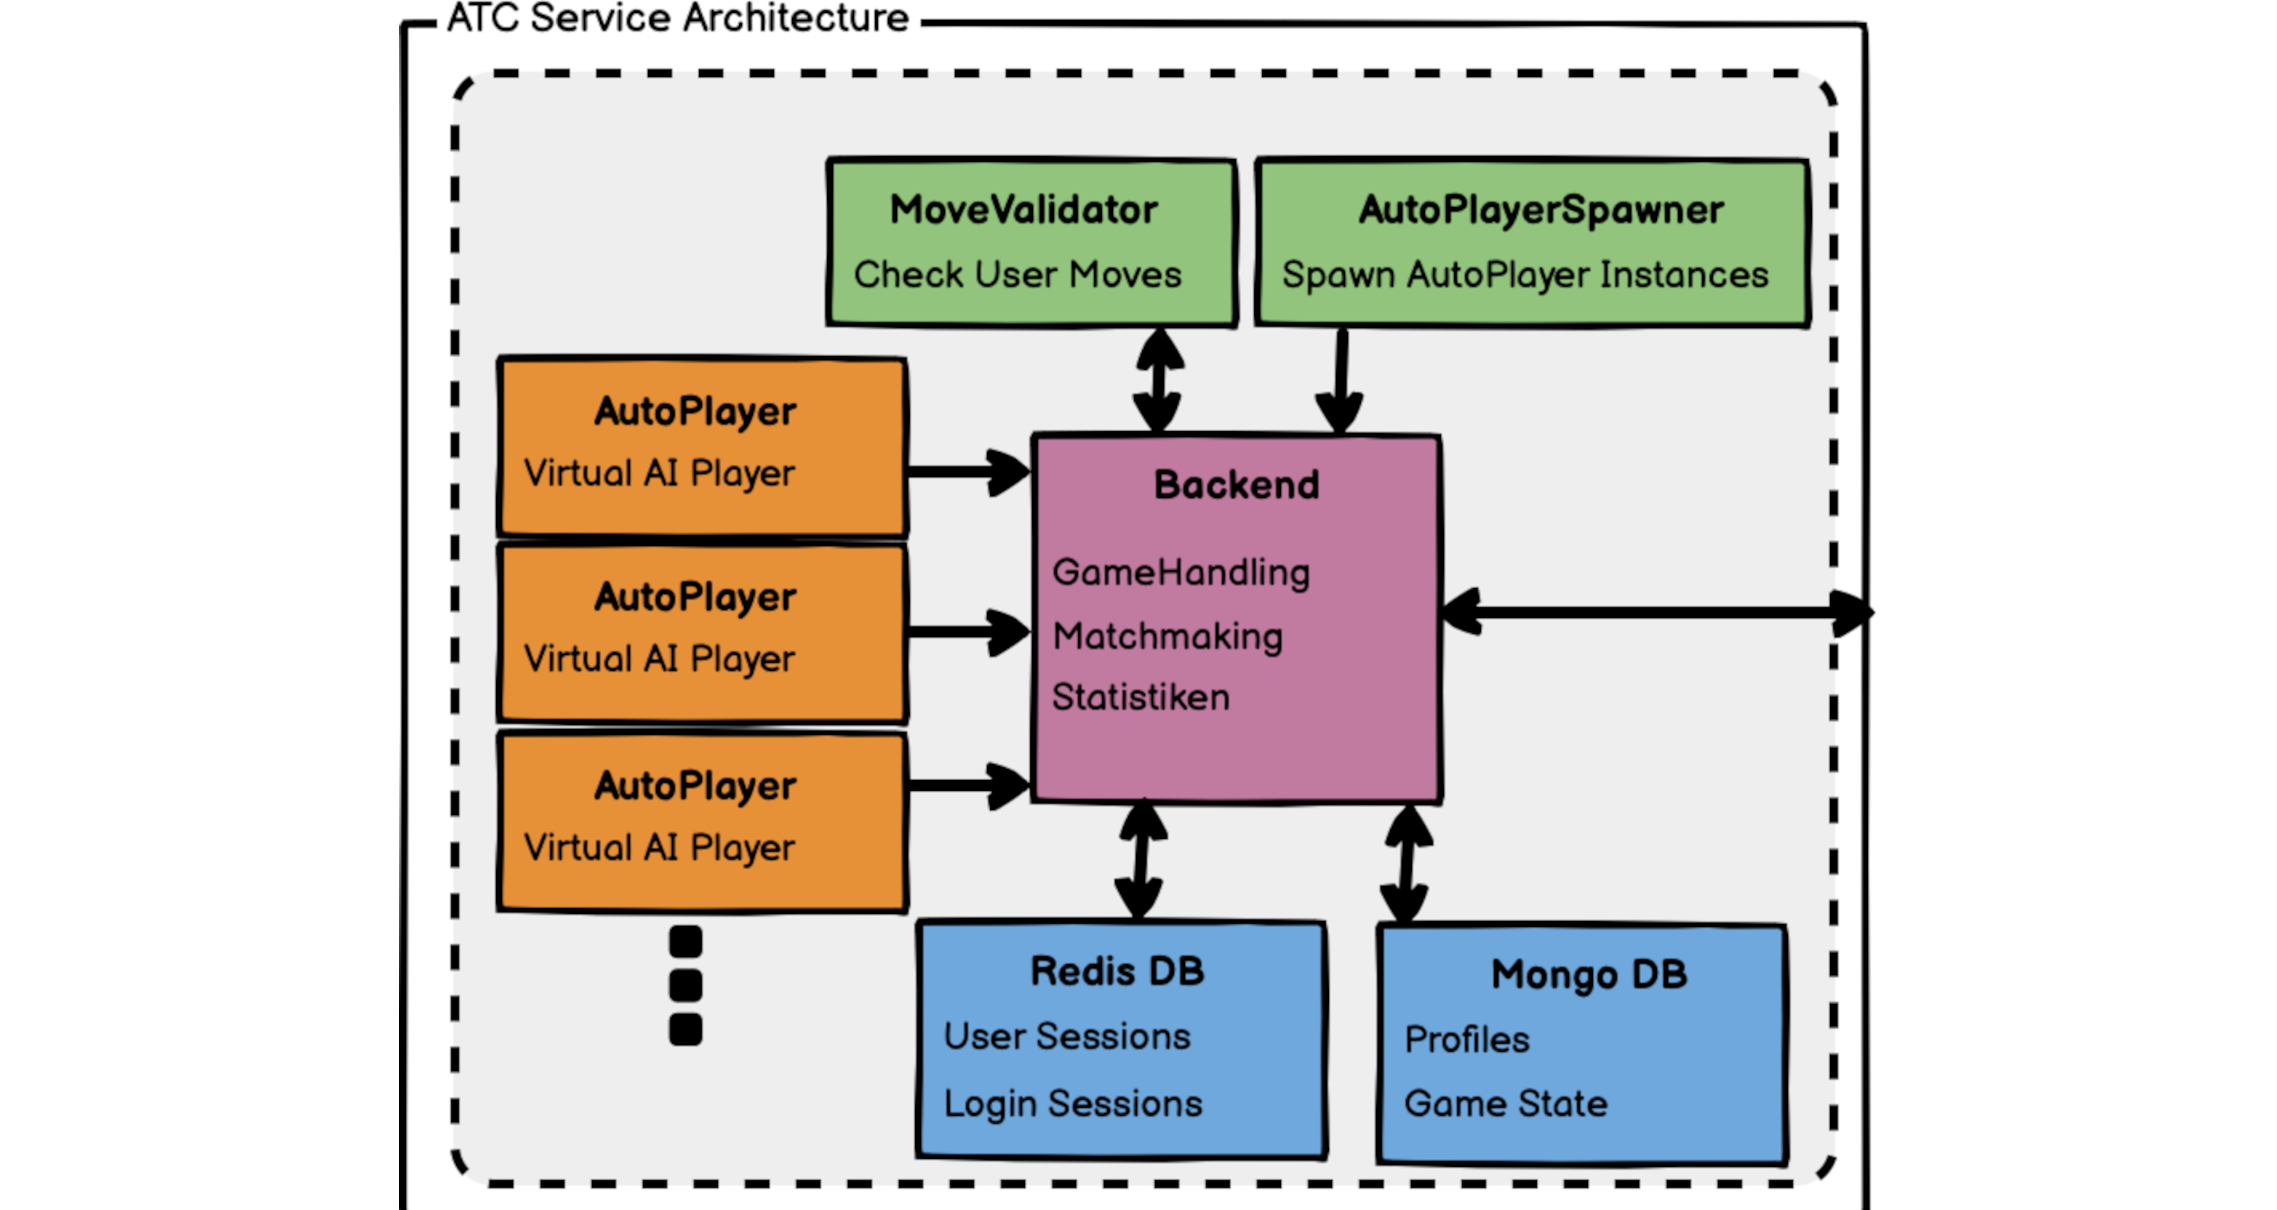
\includegraphics{images/ATC_Service_Architecture.png}
\caption{Cloud-Infrastruktur: Aufbau der Service Architecture}
\end{figure}

\hypertarget{voruxfcberlegungen}{%
\subsubsection{Vorüberlegungen}\label{voruxfcberlegungen}}

\begin{itemize}
\tightlist
\item
  welche funktionalitäten müssen abgedeckt werden
\item
  client aktivitendiagram
\end{itemize}

\hypertarget{backend}{%
\subsubsection{Backend}\label{backend}}

\begin{figure}
\centering
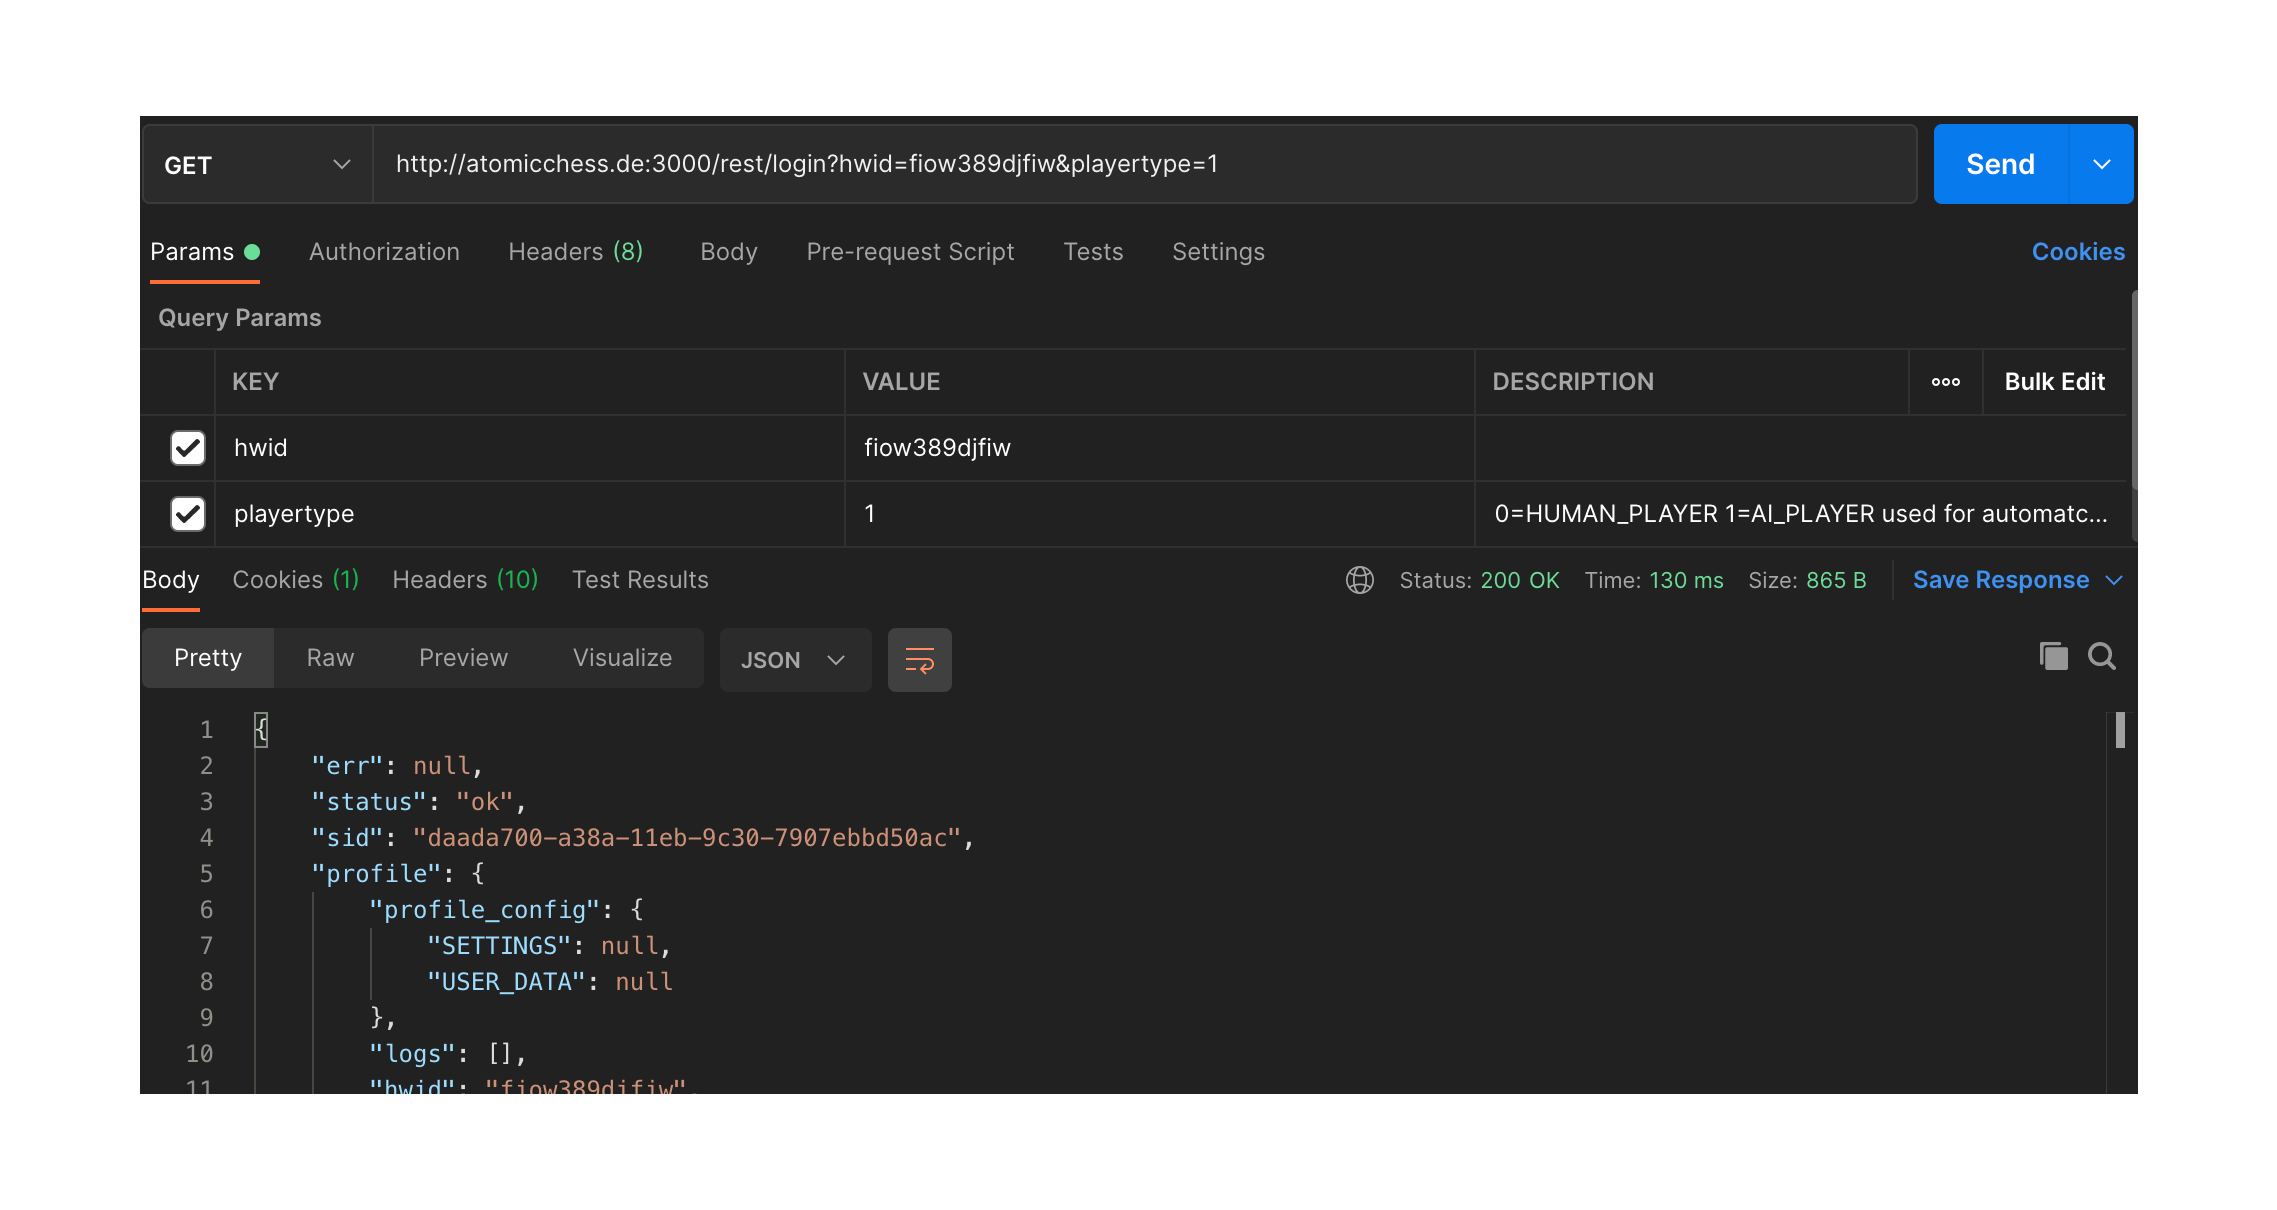
\includegraphics{images/ATC_request_example.png}
\caption{Cloud-Infrastruktur: Backend Login-Requst und Response}
\end{figure}

\begin{itemize}
\tightlist
\item
  matchmaking schachlogik
\item
  zentraler zugriffspunkt auf das System und stellt diese abi bereit
\item
  stellt spielerprofile aus datenbanken bereit bereit
\item
  authentifizierung der clients und deren sessions
\item
  weiterleitung der von spielerinteraktionen an move validator
\item
  spielfelder werden als string übermittelt = hier fen representation;
  einfach zu parsen; standart
\end{itemize}

\hypertarget{movevalidator}{%
\subsubsection{MoveValidator}\label{movevalidator}}

Der MoveValidator-Service bildet im System die eigentliche Schachlogik
ab. Die Aufgabe ist es, die vom Benutzer eingegebenen Züge auf
Richtigkeit zu überprüfen und auf daraufhin neuen Spiel-Status
zurückzugeben. Dazu zählen unter anderem das neue Schachbrett und ob ein
Spieler gewonnen oder verloren hat.

Bevor ein Spiel begonnen wird, generiert der MoveValidator das initiale
Spielfeld und bestimmt den Spieler, welcher als erstes am Zug ist.

\begin{itemize}
\tightlist
\item
  Beispiel request/repsonse
\end{itemize}

Der Backend-Service fragt einen neues Spiel an oder übergibt einen
Schachzug inkl. des Spielbretts an den Service. Der Response wird dann
vom Backend in der Datenbank gespeichert und weiter an die
Client-Devices verteilt.

Mit diesem Design ist es möglich, auch andere Spielarten im System zu
implementieren, nur hier die initialen Spielfelder generiert werden und
Züge der Spieler validiert werden müssen.

Allgemein geschieht die Kommunikation über drei API Calls.

\begin{itemize}
\item
  Auflistung der routen
\item
  generiter neues brett
\item
  python chess packge welche pesudo legal moves generiert
\item
  beispiel Requests
\end{itemize}

\hypertarget{entwicklung-webclient}{%
\subsection{Entwicklung Webclient}\label{entwicklung-webclient}}

Der Webclient wurde primär dazu entwickelt um das System während der
Entwicklung zu testen. Dieser simuliert einen autonomen Schachtisch und
verwendet dabei die gleichen \gls{http} Requests. Dieser wurde dabei
komplett in \gls{js} umgesetzt im Zusammenspiel mit \gls{html} und
\gls{css} und ist somit komplett im Browser lauffähig.

Ausgeliefert werden die statischen Dateien zur Einfachheit durch den
Backend-Service. * express router * public folder

\begin{figure}
\centering
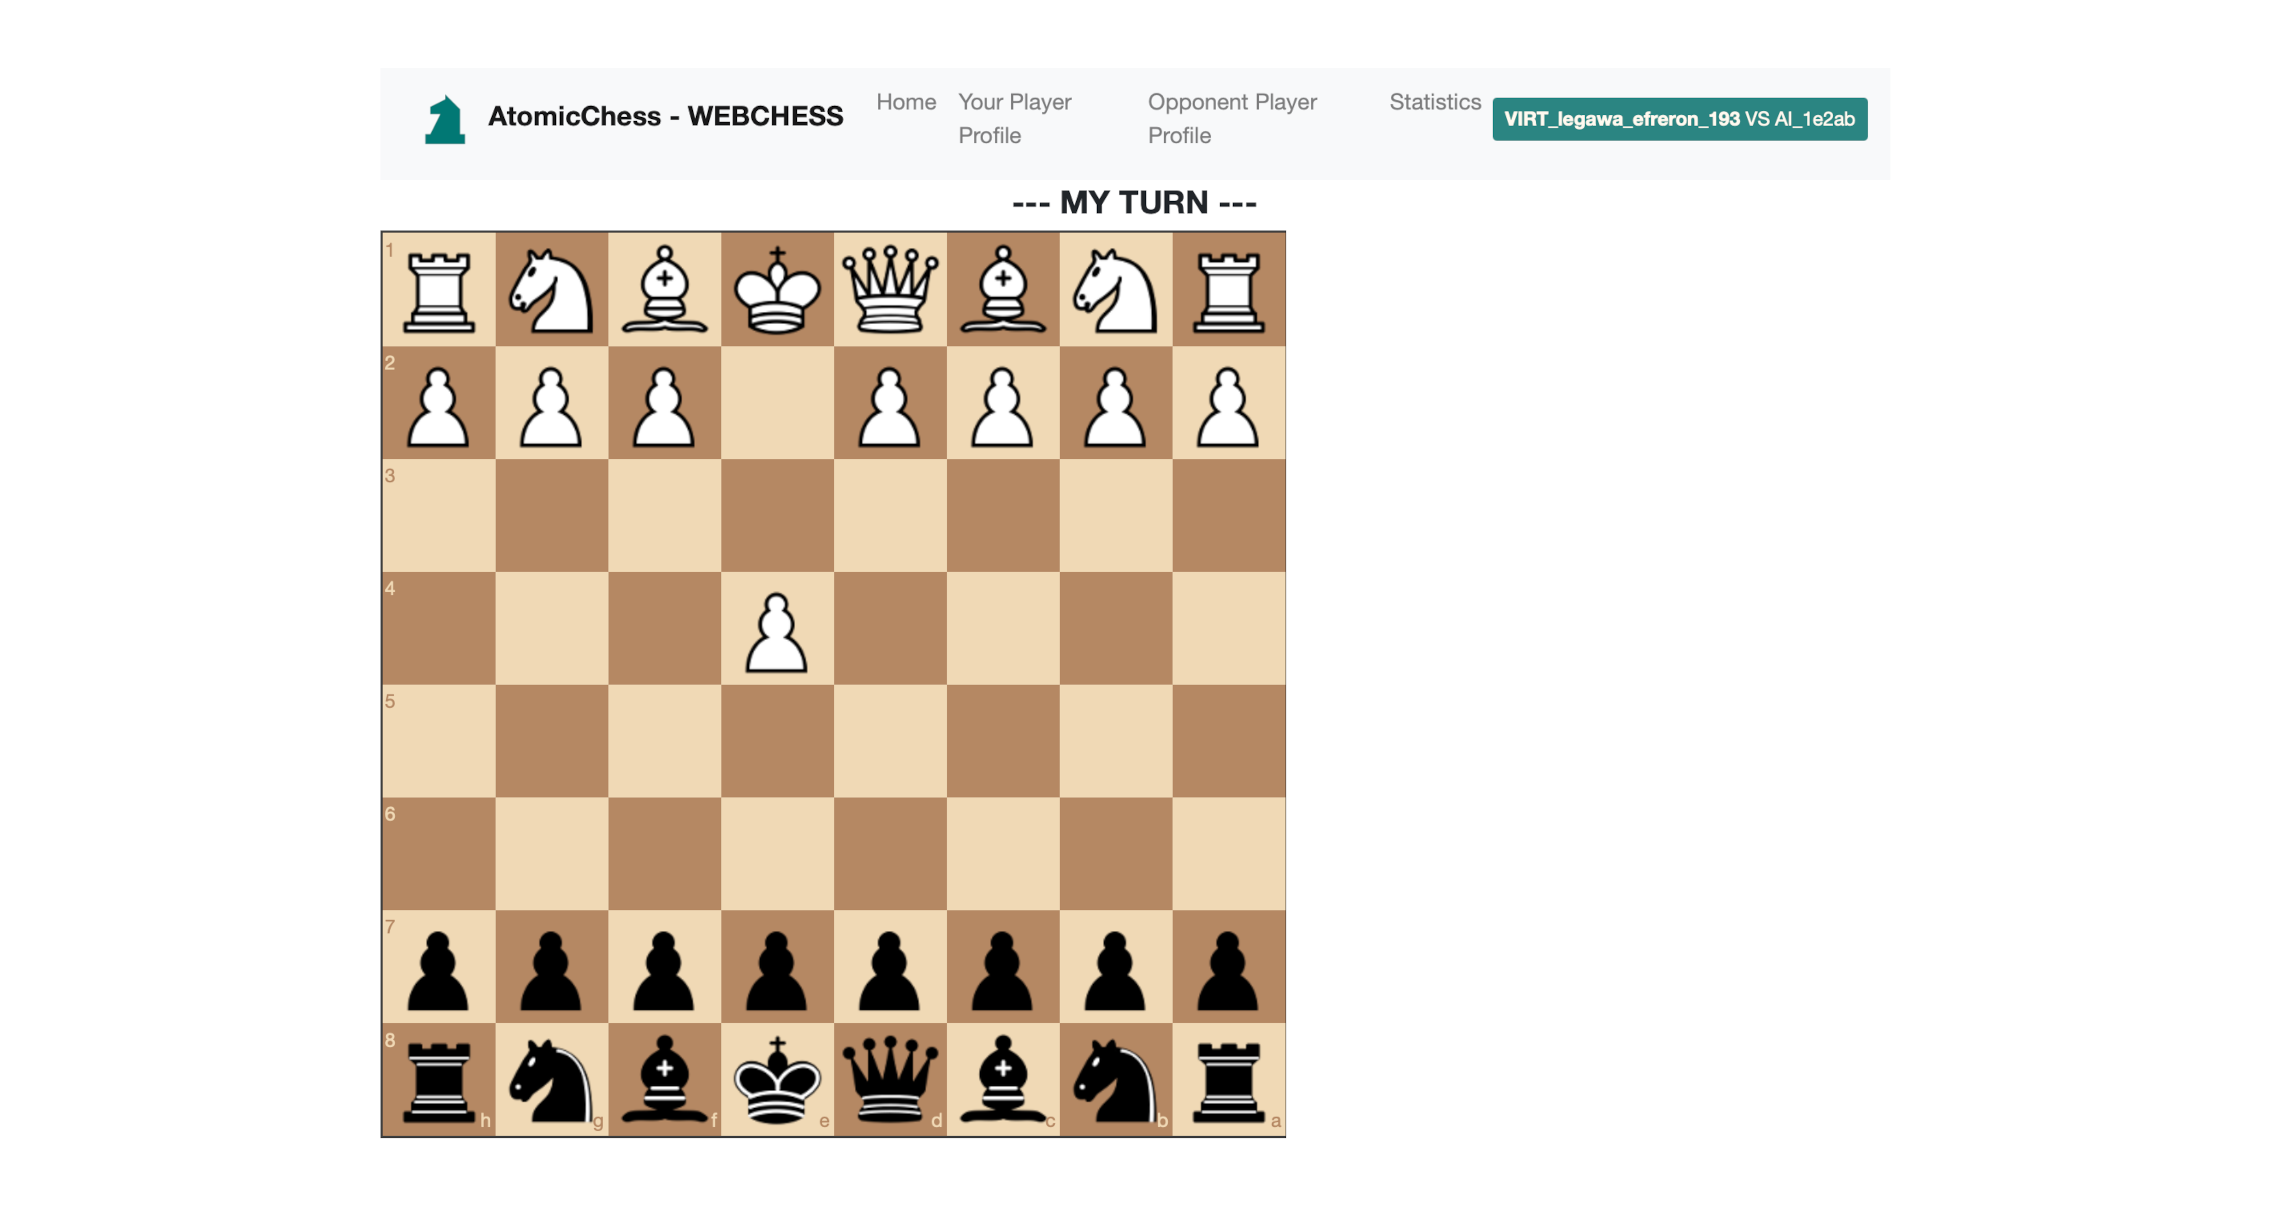
\includegraphics{images/ATC_webclient.png}
\caption{Webclient: Spielansicht}
\end{figure}

Während der Implementierung wurde der Webclient weiter ausgebaut und es
wurde weitere Features ergänzt. Dazu zählt zum einen eine Übersicht über
vergangene und aktuell laufende Spiele. In dieser können Spiele Zug um
Zug nachvollzogen werden und weitere Information über den Spielstatus
angezeigt werden. Auch ist es möglich aktuell laufende Spiele in
Echtzeit anzeigen zu lassen, somit wurde eine Livestream-Funktionaliät
implementiert.

\begin{figure}
\centering
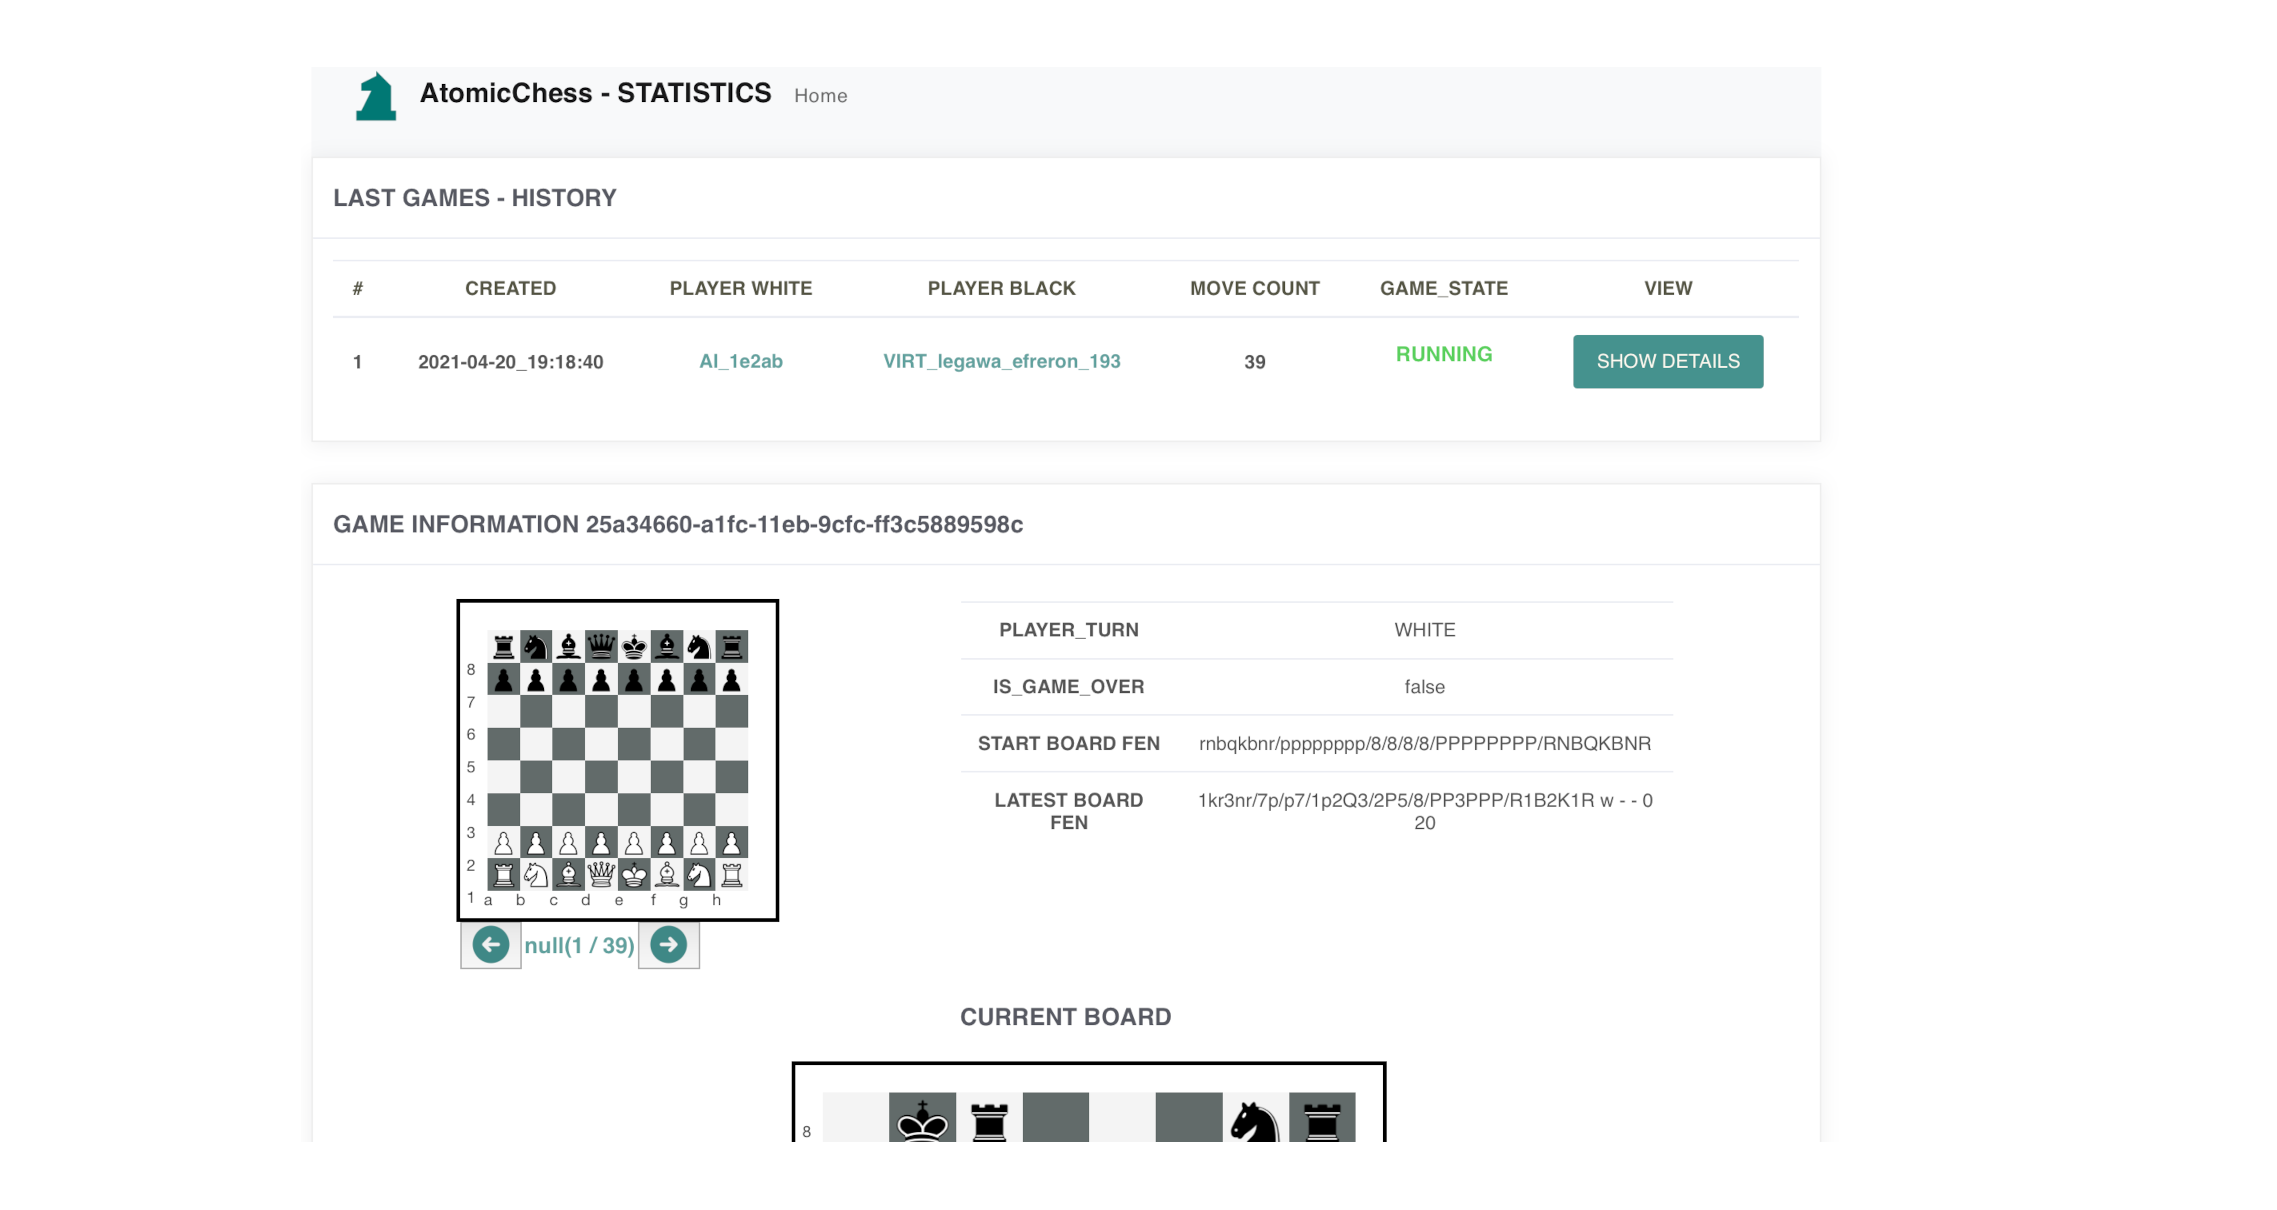
\includegraphics{images/ATC_statistics.png}
\caption{Webclient: Statistiken}
\end{figure}

\begin{itemize}
\tightlist
\item
  techstack js
\item
  backend zu testen
\item
  menschliche spieler zu simulieren
\item
  wärend der entwicklungsphase des tisches gezielt spiele simulieren zu
  können
\item
  liefert auch statistiken
\item
  wird zur einfachheit direkt aus dem abckend heraus ausgeliefert da nur
  statisches html/js/class
\end{itemize}

\hypertarget{autoplayer}{%
\subsubsection{AutoPlayer}\label{autoplayer}}

Der AutoPlayer-Service stellt den Computerspieler bereit. Jede
Service-Instanz stellt einen virtuellen Spieler bereit, welcher die
gleiche Schnittstellen wie der Webclient oder der autonme Schachtisch
verwendet. Die einzige Änderung an den verwendeten \gls{rest}-Calls ist
der Login-Requst. Hier wird das \passthrough{\lstinline!playertype!}
Flag gesetzt welches den Spieler als Computerspieler gegenüber des
Systems authentifiziert. Somit wird dieser wärend des
Matchmaking-Prozesses erst für ein Match ausgewählt, wenn kein anderer
Spieler mehr zur Verfügung steht, welcher vom Typ Webclient oder
autonomer Schachtisch ist. Somit ist gewährleistet, dass immer zuerst
die Menschlichen-Spieler ein Spiel beginnen.

Eine weitere Modifikation ist die verwendung einer Schach-AI, da dieser
Service als Computerspieler agieren soll. Hierzu kam die Open-Source
Chess Engine Stockfish\cite{stockfish} in der Version 11 zum
Einsatz. Die Stockfish-Engine bietet noch weitere Features, als nur die
nöchst besten Züge zu einem gegebenen Schachbrett zu ermitteln. Sie kann
auch genutzt werden um Züge zu klassifizieren und bietet
Analysemöglichkeiten für Spielstellungen.

Die AutoPlayer-Instanz kommuniziert über das \gls{uci}
Protokoll\cite{uciprotocol} mit der Executable der Stockfish-Engine.
Dieses Protokoll wird in der Regel von Schach-Engines um mit einer
\gls{gui} zu Kommunizieren und die Kommunikation erfolgt über
Klartextbefehle. Um das aktuelle Spielbrett in der Engine zu setzten
wird dieses in der \gls{fen} Notation mit dem Prefix
\passthrough{\lstinline!position fen!} als Klartext an die Engine
übergben.

Im Kontext des AutoPlayer-Service wird der Engine nur das aktuelle
Spielbrett übermittelt und der nächst beste Zug ausgelsen. Dies wird
Ausgeführt, wenn der AutoPlayer am Zug ist. Nachdem die Engine einen
passenden Zug gefunden hat, wird das Ergebnis über den
\passthrough{\lstinline!make\_move!} \gls{rest}-API Call übermittelt.

Wenn das Match beendet wird, beendet sich auch die Service-Instanz.
Diese wird jedoch wieder gestartet wenn die Anzahl der zur Verfügung
stehenden Computerspieler unter einen definierten Wert fallen. Somit ist
dafür gesorgt, dass das System nicht mit ungenutzen AutoPlayer-Instanzen
gebremst wird. Diese Anzahl ist in der Backend-Configuration frei
wählbar und kann je nach zu erwartenen Aufkommen angepasst werden.

\begin{figure}
\centering
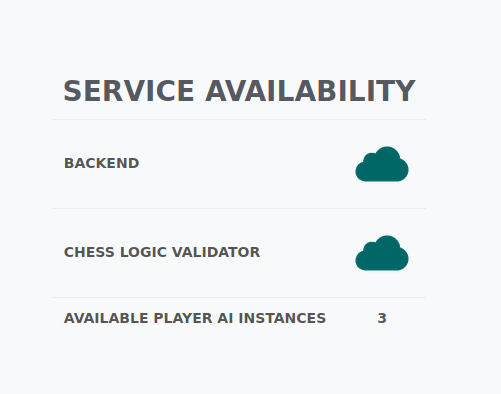
\includegraphics{images/ai_player_count.png}
\caption{Webclient: Anzahl der aktiven, sich nicht im Spiel befindenen
AutoPlayer-Service-Instanzen}
\end{figure}

Allgemein skaliert das System durch diese Art der Ressourcenverwaltung
auch auf kleinen Systemen sehr flexibel. Durch die Art der
Implementierung, dass sich der AutoPlayer-Service wie ein normaler
Spieler verhält, sind auch andere Arten des Computerspieler möglich. So
ist es zum Beispiel möglich, die Spielstärke je Spieler anzupassen oder
einen Computerspieler zu erstellen, welcher nur zufällige Züge zieht.

Ein weiterer Anwendungsfall für den AutoPlayer-Service, ist das Testen
des weiteren Systems insbesondere des Backend-Service. Durch das
Matching von zwei AutoPlayer-Instanzen, können automatisierte test
Schachpartien ausgeführt werden um die Funktionsfähigkeit des restlichen
Systems zu testen. Diese Feature wurde insbesondere bei der Entwicklung
des Webclienten und der Steuerungssoftware für den autonomen Schachtisch
verwendet.

\hypertarget{authetifizierung}{%
\subsection{Authetifizierung}\label{authetifizierung}}

\begin{itemize}
\tightlist
\item
  authetifizierung
\item
  https only
\item
  Zertifikate auf Clientseite geniert jedoch nicht Abgefragt
\end{itemize}

\hypertarget{embedded-system-software}{%
\section{Embedded System Software}\label{embedded-system-software}}

\begin{itemize}
\tightlist
\item
  Hauptsoftware zur Steuerung der Elektrik/Mechanik
\item
  Kommunikation mit dem Cloud-Server
\end{itemize}

\hypertarget{ablaufdiagramm}{%
\subsection{Ablaufdiagramm}\label{ablaufdiagramm}}

\begin{itemize}
\item
  dummer Client
\item
  Synchronisierung von gegeben Schachfeld mit dem lokalen Schachfeld
\item
  vier Schritte (enfernen, bewegen, hinzufügen, bewegen)
\end{itemize}

\begin{figure}
\centering
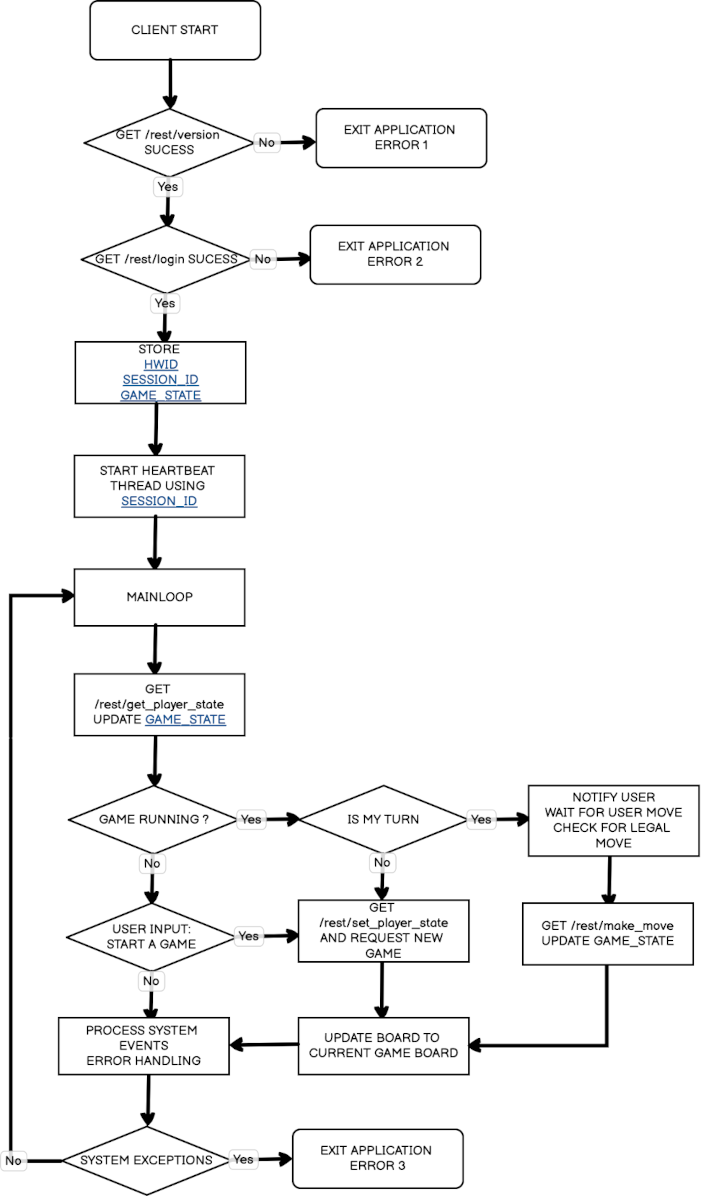
\includegraphics{images/ATC_gameclient_statemachiene.png}
\caption{Embedded System Software: Ablaufdiagramm}
\end{figure}

\hypertarget{figur-bewegungspfadberechnung}{%
\subsection{Figur
Bewegungspfadberechnung}\label{figur-bewegungspfadberechnung}}

\begin{itemize}
\tightlist
\item
  Algorithmus zur Umsetzung eines Schachzugs
\item
  Auftrennung in current und target Board
\end{itemize}

\hypertarget{schachfeld-scan-algorithmus-zur-erkennung-von-schachzuxfcgen}{%
\subsection{Schachfeld Scan Algorithmus zur Erkennung von
Schachzügen}\label{schachfeld-scan-algorithmus-zur-erkennung-von-schachzuxfcgen}}

\begin{figure}
\centering
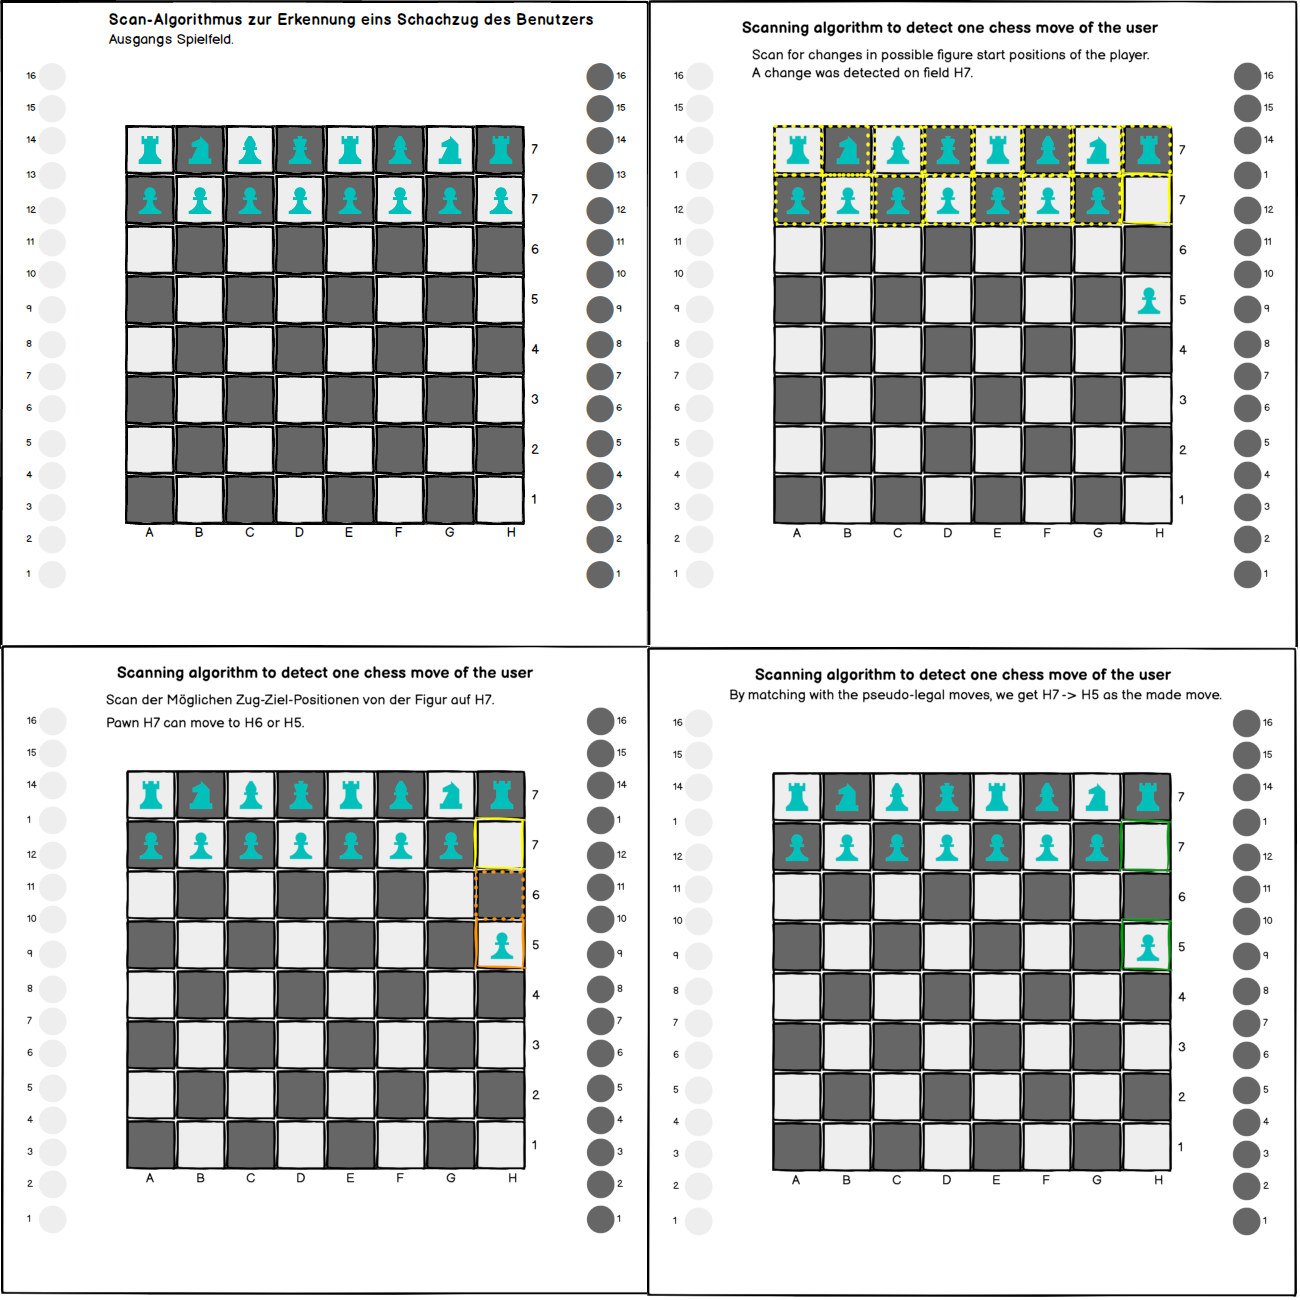
\includegraphics{images/ATC_ChessMoveAlgorithm.png}
\caption{Embedded System Software: Schachfeld Scan Algorithmus Ablauf}
\end{figure}

\begin{itemize}
\tightlist
\item
  Benutzer bestätigt dass er Schachzug gemacht hat
\item
  Ermittlung des getätigten Schachzug
\item
  Scan der Schachfeld-Veränderungen, durch Vergleich des vorherigen
  Schachfelds und der möglichen Züge
\end{itemize}

\hypertarget{userinterface}{%
\subsection{Userinterface}\label{userinterface}}

\begin{figure}
\centering
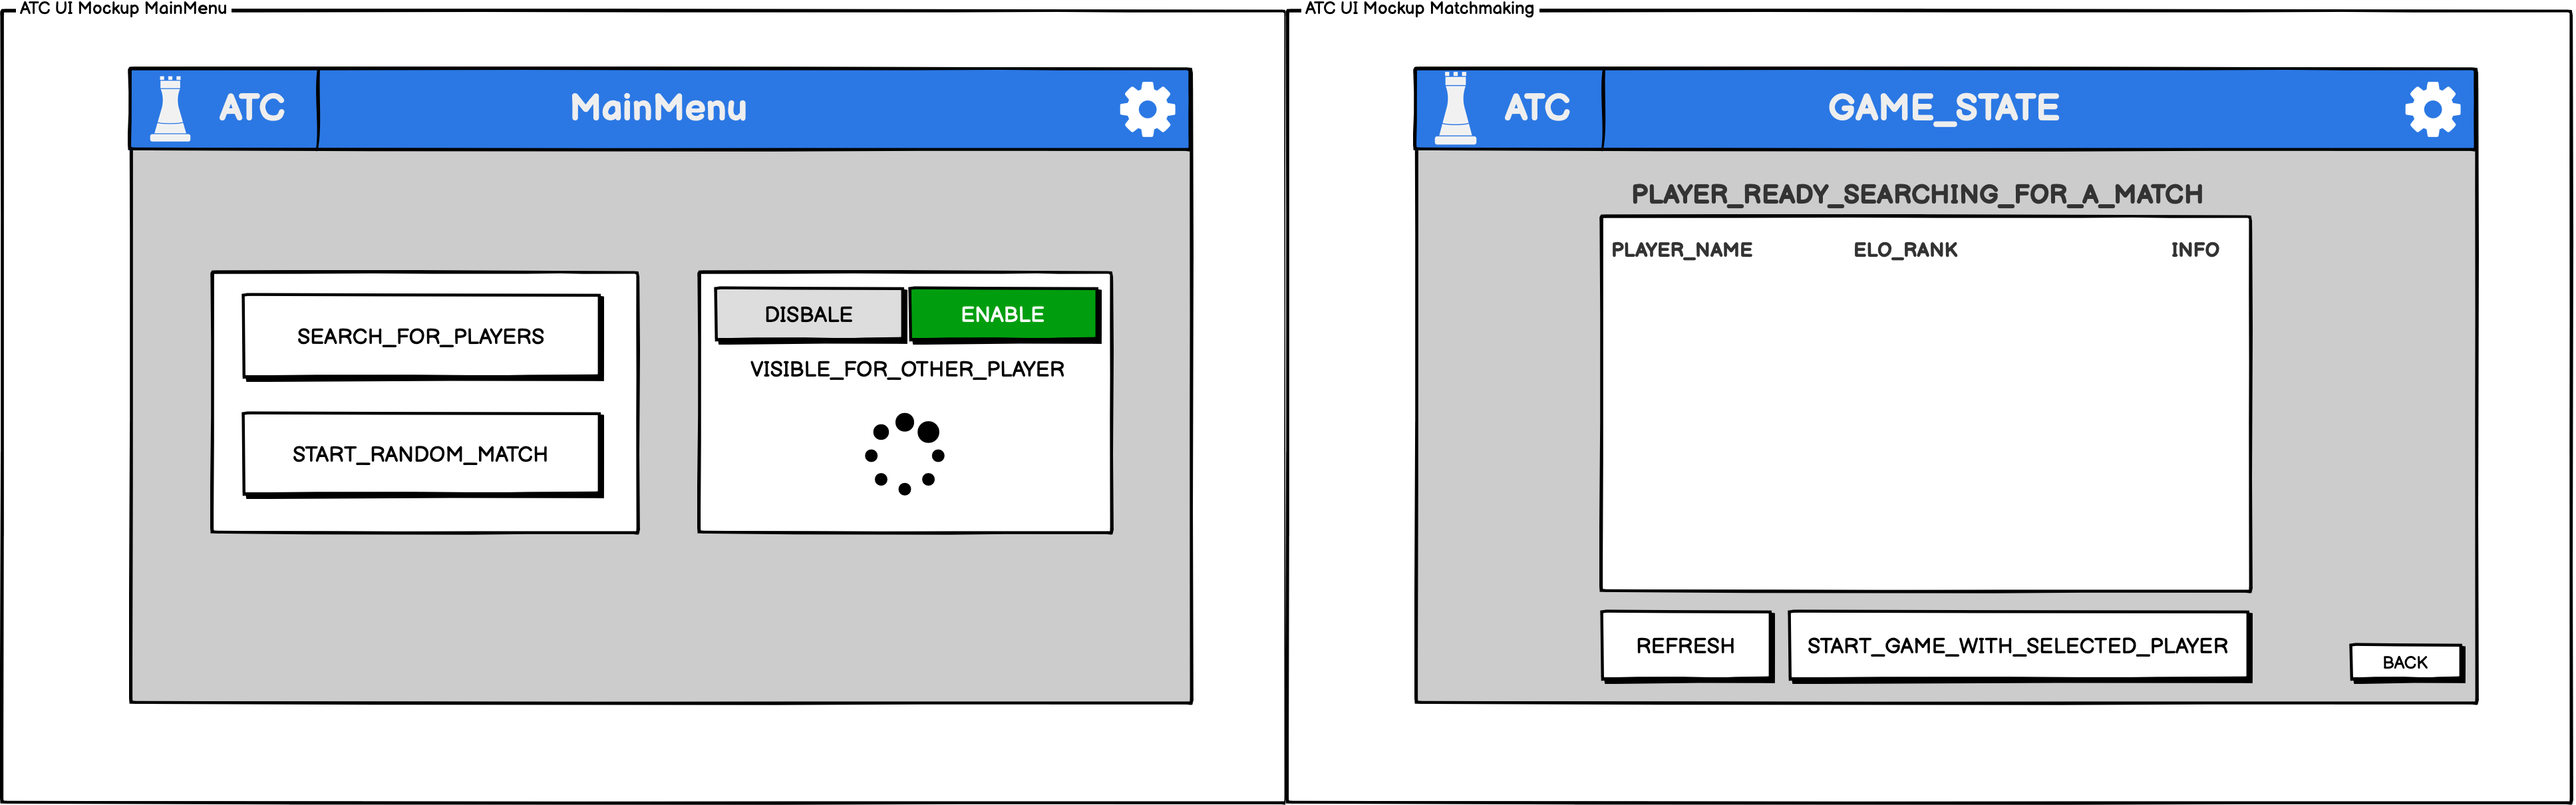
\includegraphics{images/ATC_Gui.png}
\caption{Embedded System Software: User-Interface Mockup}
\end{figure}

\begin{itemize}
\tightlist
\item
  QT Quick UI, als Package in Buildroot integriert
\item
  IPC Bibliothek zur Kommunikation mit der controller-Software Instanz
\item
  JSON basiert =\textgreater{} einfaches Debugging
\item
  Steuerung über andere Endgeräte möglich z.B Handy-App welche im selben
  Netzwerk befindet.
\end{itemize}

\hypertarget{fazit}{%
\section{Fazit}\label{fazit}}

\begin{itemize}
\tightlist
\item
  mit am weitesten forgeschrittener open-source autonomes Schachtisch
  Projekt
\end{itemize}

\hypertarget{ausblick}{%
\subsection{Ausblick}\label{ausblick}}

\begin{itemize}
\tightlist
\item
  Einbindung in existeirende Schach-Clouds z.B. https://lichess.org/
\item
  user-port für Erweiterungen (z.B. DGT Schachur)
\end{itemize}
